\documentclass[journal]{IEEEtran}
\usepackage{amsmath,amssymb}
\usepackage{amsthm}
\usepackage{booktabs}
\usepackage{tikz}
\usepackage{pgfplots}
\pgfplotsset{compat=1.16}
\usetikzlibrary{arrows.meta,positioning,calc,trees}

\newtheorem{theorem}{Theorem}
\newtheorem{lemma}{Lemma}
\newtheorem{proposition}{Proposition}
\newtheorem{corollary}{Corollary}
\theoremstyle{definition}
\newtheorem{remark}{Remark}

\newcommand{\Hh}{\mathrm H_2}
\newcommand{\kp}{\kappa}
\newcommand{\lgg}{\log_2}
\newcommand{\CC}{C}
\newcommand{\lam}{\lambda}
\newcommand{\cthree}{c_3}
\newcommand{\cS}{\mathcal{S}}
\newcommand{\cP}{\mathcal{P}}
\newcommand{\cD}{\mathcal{D}}

\title{A Gallager-Type Redundancy Bound for\\ Binary Shannon-Fano Coding}
\author{Kamila~Szewczyk%
\thanks{K. Szewczyk is with the Algorithmic Bioinformatics group,
Saarland University, Saarbr\"ucken, Germany
(e-mail: szewczyk@cs.uni-saarland.de).}}

\begin{document}
\maketitle

\begin{abstract}
Kraj\v{c}i, Liu, Mike\v{s}, and Moser proved in 2015 that the redundancy of
binary Shannon-Fano coding is always below one bit. We sharpen this to a bound
depending on the largest source probability $p_1$: an explicit seven-piece
envelope $R<f(p_1)$. The envelope equals the exact supremum of $R$ given $p_1$
for every $p_1\ge\tfrac12$ and on a subinterval below $\tfrac13$, and gives the
cap $R<\tfrac52-\tfrac56\log_2 5=0.5651$ for $p_1<\tfrac12$. It is the first
$p_1$-dependent redundancy bound for Fano codes. The method is more sophisticated
than the approach typical for Huffman codes:
Fano trees are built top-down by contiguous balanced splits and lack the
sibling property. From the $R<1$ theorem the rest follows from the Fano
recursion, through a min-corrected affine potential and a no-burial lemma. Every
scalar inequality in the proof reduces to a comparison of integer powers.
\end{abstract}

\begin{IEEEkeywords}
Shannon-Fano coding, source coding, redundancy, prefix codes, Huffman codes,
entropy.
\end{IEEEkeywords}

\IEEEpeerreviewmaketitle

\section{Introduction}\label{sec:intro}

\IEEEPARstart{B}{inary} Shannon--Fano coding \cite{Shannon48,Fano49} sorts the
source symbols by probability and recursively splits the sorted list into two
contiguous blocks of as nearly equal probability as possible, one code bit per
split. Unlike the bottom-up Huffman construction \cite{Huffman52} it need not be
optimal. Because the blocks are contiguous the code preserves the sorted order,
so it is an \emph{alphabetic} code \cite{GilbertMoore59}, whose optimum is the
Hu--Tucker code \cite{HuTucker71}. Following \cite{CoverThomas06} we reserve the
name \emph{Shannon--Fano} for this top-down split code, as opposed to the
Shannon--Fano--Elias code.

The efficiency of a code is its \emph{redundancy}
$R=\mathbb E[\ell]-\mathrm H(p)$, the expected codeword length minus the
entropy. For \emph{Huffman} codes, $R$ has long been bounded in terms of the
largest symbol probability $p_1$. Gallager \cite{Gallager78} introduced the
sibling property and proved $R<p_1+0.086$, reproved more simply by Ye and Yeung
\cite{YeYeung02}; Johnsen \cite{Johnsen80} improved the estimate for
$p_1\ge0.4$; and Capocelli, Giancarlo, and Taneja
\cite{CapocelliGiancarloTaneja86}, Capocelli and De~Santis
\cite{CapocelliDeSantis89,CapocelliDeSantis91}, Montgomery and Abrahams
\cite{MontgomeryAbrahams87}, and Manstetten \cite{Manstetten92} determined the
exact worst-case Huffman redundancy as a function of $p_1$. All of these use the
sibling property of Huffman trees, which orders the nodes by weight in sibling
pairs.

Fano codes have been analysed less. Rissanen \cite{Rissanen73} and Horibe
\cite{Horibe77} bounded weight-balanced trees, of which a Fano tree is one
($\mathrm H\le W\le\mathrm H+3$, later sharpened), and Nakatsu \cite{Nakatsu91}
bounded the redundancy of alphabetic codes; Kraj\v{c}i, Liu, Mike\v{s}, and
Moser \cite{Krajci15} proved the universal estimate $R<1$ for Fano coding. A
$p_1$-dependent bound of Gallager type has been missing. The
obstruction is structural: a Fano tree is built top-down by contiguous balanced
cuts and does not satisfy the sibling property, so the subtrees in the recursion
need not be near-uniform and the Huffman block estimates do not carry over.

\subsection*{Contributions}
We prove the first $p_1$-dependent redundancy bound for binary Shannon--Fano
coding:
\begin{itemize}
\item a seven-piece envelope $R<f(p_1)$ (Theorem~\ref{thm:main}) that sharpens
  $R<1$ \cite{Krajci15} for every $p_1$ and gives the cap
  $R<K=\tfrac52-\tfrac56\lgg5=0.5651$ for $p_1<\tfrac12$;
\item tightness: the envelope is the exact supremum of $R$ given $p_1$ on
  $[\tfrac12,1)$ and on $[b_2,\tfrac13)$
  (Propositions~\ref{prop:tight} and~\ref{prop:tight-q});
\item a proof from the Fano recursion alone, using the min-corrected potential
  $\Psi=p_1+\CC-\lam p_n$ and a no-burial lemma that puts the largest symbol at
  depth two on $[\tfrac14,\tfrac13)$;
\item a reduction of every scalar inequality in the proof to a comparison of
  integer powers, so the argument is elementary and self-contained
  (Appendix~\ref{app:cert}).
\end{itemize}

\subsection*{Organization}
Section~\ref{sec:model} fixes the construction and notation.
Section~\ref{sec:main} states the envelope and its tightness.
Section~\ref{sec:outline} outlines the proof; the details are in the appendices.
Section~\ref{sec:disc} discusses tightness and the limits of the method.

\section{Shannon--Fano Coding and the Fano Recursion}\label{sec:model}

A \emph{source} is a probability vector $p=(p_1,\dots,p_n)$ with
$p_1\ge\cdots\ge p_n>0$ and $\sum_i p_i=1$. The binary \emph{Shannon--Fano} code
\cite{Shannon48,Fano49} is the leaf code of the tree built by the following
recursion on contiguous blocks of the sorted list. A block consisting of a single
symbol is a leaf. A block $\{i,\dots,j\}$ of mass $M=\sum_{t=i}^{j}p_t$ is split
after a position $k$ ($i\le k<j$) into a left part $\{i,\dots,k\}$ (code bit $0$)
and a right part $\{k+1,\dots,j\}$ (code bit $1$), where $k$ minimises the
\emph{imbalance} $|m_L-m_R|$, $m_L=\sum_{t=i}^{k}p_t$, $m_R=M-m_L$; then recurse
on the two parts. We fix the convention that ties among minimising cuts are
broken toward the smaller left part; the code, and hence $R$, is then well
defined. The convention enters only through the exact isolation criterion of
Lemma~\ref{lem:iso} \textup{(}at $2p_1+p_2=1$\textup{)} and its uses; the
uniform cases of \S\ref{ss:unif} and the extremal families of
Propositions~\ref{prop:tight} and~\ref{prop:tight-q} are verified for every
minimising cut.

Let $\ell_i$ denote the depth of symbol $i$ in this tree (its codeword length),
$\mathbb E[l]=\sum_i p_i\ell_i$ the expected length, $\mathrm H(p)=-\sum_i p_i\lgg p_i$ the entropy, and $R = R(p) := \mathbb E[l]-\mathrm H(p)$
the \emph{redundancy}. Since every internal node of the tree has two children,
the Kraft sum is exactly $1$, so $R=\sum_i p_i\bigl(\ell_i+\lgg p_i\bigr)
=\mathrm D\bigl(p\,\|\,2^{-\ell}\bigr)\ge0$, where $\mathrm D$ denotes
Kullback--Leibler divergence.

The construction is recursive: if the root splits into a left part of mass $a$
and a right part of mass $1-a$, with renormalised children $B_L,B_R$, then
$R=\bigl(1-\Hh(a)\bigr)+a\,R(B_L)+(1-a)\,R(B_R)$ (Lemma~\ref{lem:rec}).
Figure~\ref{fig:trees} shows the two root behaviours the proof turns on: either
the root isolates the largest symbol at depth one, or it does not, in which case
on $[\tfrac14,\tfrac13)$ the largest symbol still sits at depth exactly two.

\begin{figure}[t]
\centering
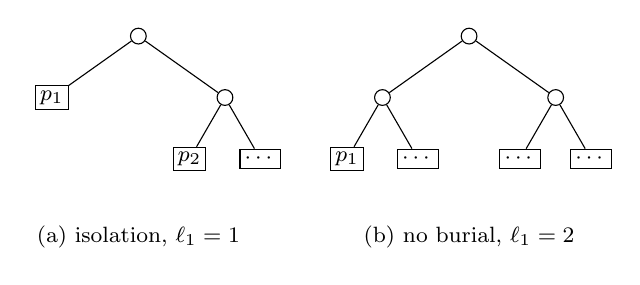
\begin{tikzpicture}[level distance=7.8mm, level 1/.style={sibling distance=22mm},
  level 2/.style={sibling distance=9mm},
  every node/.style={font=\footnotesize},
  inode/.style={circle,draw,inner sep=1.3pt,minimum size=2mm},
  leaf/.style={rectangle,draw,inner sep=1.7pt}]
\begin{scope}
\node[inode]{}
  child {node[leaf]{$p_1$}}
  child {node[inode]{}
    child {node[leaf]{$p_2$}}
    child {node[leaf]{$\cdots$}}};
\node at (0,-2.55){(a) isolation, $\ell_1=1$};
\end{scope}
\begin{scope}[xshift=42mm]
\node[inode]{}
  child {node[inode]{}
    child {node[leaf]{$p_1$}}
    child {node[leaf]{$\cdots$}}}
  child {node[inode]{}
    child {node[leaf]{$\cdots$}}
    child {node[leaf]{$\cdots$}}};
\node at (0,-2.55){(b) no burial, $\ell_1=2$};
\end{scope}
\end{tikzpicture}
\caption{The two root behaviours. When $2p_1+p_2\ge1$ the root splits the leader
off on its own (depth one); when $p_1\in[\tfrac14,\tfrac13)$ it cannot, but the
leader is still a leaf at depth exactly two (Lemma~\ref{lem:noburial-q}).}
\label{fig:trees}
\end{figure}

Throughout, $\mathrm I(p):=-p\lgg p$ \textup{(}$\mathrm I(0)=0$\textup{)},
$\Hh(p):=\mathrm I(p)+\mathrm I(1-p)$ is the binary entropy function
\textup{(}concave, $\Hh(0)=\Hh(1)=0$, $\Hh(\tfrac12)=1$\textup{)}, and for a
nonnegative vector we write
$\mathrm H(p_1,\dots,p_k):=\sum_i \mathrm I(p_i)$.

\section{Main Result}\label{sec:main}

The envelope is built from the balance function
\[
\begin{aligned}
  \kp(d)&\ :=\ 1-\Hh\!\Bigl(\tfrac{1+d}{2}\Bigr)\quad(d\in[-1,1]),\\
  \cthree&\ :=\ \kp(\tfrac13)\ =\ \tfrac53-\lgg3 .
\end{aligned}
\]
The function $\kp$ is even and convex, with $\kp(0)=0$ and $\kp(\pm1)=1$. The
constants of the paper are built from $\cthree$ and from the second value
$\kp(\tfrac15)=\tfrac75+\tfrac35\lgg3-\lgg5$:
\begin{equation}\label{eq:constants}
\begin{aligned}
  \lam&\ :=\ 1+5\,\kp(\tfrac15)\ =\ 8+3\lgg3-5\lgg5,\\
  \CC&\ :=\ \cthree+\frac{\lam-1}{3} .
\end{aligned}
\end{equation}
Substituting the closed forms, the $\lgg3$-terms cancel identically:
\begin{equation}\label{eq:cancel}
  \CC=4-\tfrac53\lgg5 .
\end{equation}
Numerically $\cthree=0.081704\ldots$, $\lam=1.145247\ldots$, and
$\CC=0.130119\ldots$. All inequalities between the explicit constants below
reduce to comparisons of products of powers of small integers; we use such facts
without further comment. Put
\[
  K:=\frac{1+\CC}{2}=\frac52-\frac56\lgg5,\qquad
  V(x):=2-x-\Hh(x),
\]
\[
\begin{aligned}
  W_{\mathrm{iso}}(x)&:=1-\Hh(x)+(1-x)K,\\
  F_\ell(x)&:=\frac{5-x}{3}+\frac{2-x}{3}\CC
  -\mathrm H\Bigl(x,\frac{1-2x}{3},\frac{2-x}{3}\Bigr),
\end{aligned}
\]
and
\[
\begin{aligned}
  \Pi(x)&:=\frac32+\frac{\CC}{2}-x-\mathrm I(x)-\mathrm I\left(\frac12-x\right),\\
  \Theta(x)&:=\frac{4+2x}{3}+\frac{2(1-x)}{3}K
   -\mathrm H\Bigl(x,\frac{1-x}{3},\frac{2(1-x)}{3}\Bigr),\\
  N(x)&:=3-3x-\mathrm H(x,x,x,1-3x).
\end{aligned}
\]
Let $r_1,q_2,r_*$ be defined as the unique zeros
\[
  \begin{aligned}
  0&=\Hh(r_1)-\Bigl(\frac53\lgg5-2\Bigr)r_1
      -\lgg3-\frac43+\frac{10}{9}\lgg5,\\
   &\qquad r_1\in(\tfrac14,\tfrac13),\\
  0&=2\mathrm I(q_2)+\mathrm I(1-2q_2)+2q_2-\lgg3-\frac59\lgg5+\frac23,\\
   &\qquad q_2\in(\tfrac25,\tfrac12),\\
  0&=\Hh(r_*)+\Bigl(5-\frac53\lgg5\Bigr)r_*-\frac52+\frac56\lgg5,\\
   &\qquad r_*\in(0,\tfrac16).
  \end{aligned}
\]
Then the three switching constants are
\[
  b_1=\frac{1-2r_1}{2(1-r_1)},\qquad
  b_2=\frac{q_2}{1+q_2},\qquad
  p^*=\frac{1-3r_*}{2-3r_*}.
\]
The substitutions
$r=(\tfrac12-x)/(1-x)$, $q=x/(1-x)$, and
$r=(1-2x)/(3(1-x))$ convert respectively $\Pi=\Theta$, $\Theta=N$, and
$W_{\mathrm{iso}}=F_\ell$ into these zero equations.
Lemmas~\ref{lem:cross} and~\ref{lem:cross-q} prove the needed uniqueness
statements. Numerically
$b_1=0.3190251\ldots$, $b_2=0.3196323\ldots$, and
$p^*=0.415798\ldots$.

Our main result is:

\begin{theorem}[Main theorem]\label{thm:main}
For every source with $n\ge2$ symbols,
\[
   \boxed{\ \ R\ <\ \begin{cases}
   p_1+\CC, & 0<p_1<\tfrac14,\\[2pt]
   \Pi(p_1), & \tfrac14\le p_1\le b_1,\\[2pt]
   \Theta(p_1), & b_1\le p_1\le b_2,\\[2pt]
   N(p_1), & b_2\le p_1<\tfrac13,\\[2pt]
   W_{\mathrm{iso}}(p_1), & \tfrac13\le p_1\le p^*,\\[2pt]
   F_\ell(p_1), & p^*\le p_1<\tfrac12,\\[2pt]
   V(p_1), & \tfrac12\le p_1<1,
   \end{cases}\ \ }
\]
with the curves $\Pi,\Theta,N,W_{\mathrm{iso}},F_\ell,V$ and the switching
points $b_1<b_2$, $p^*$ as defined above.
Consequently $R<K=\tfrac52-\tfrac56\lgg5$ for every source with
$p_1<\tfrac12$.
\end{theorem}

\begin{figure}[t]
\centering
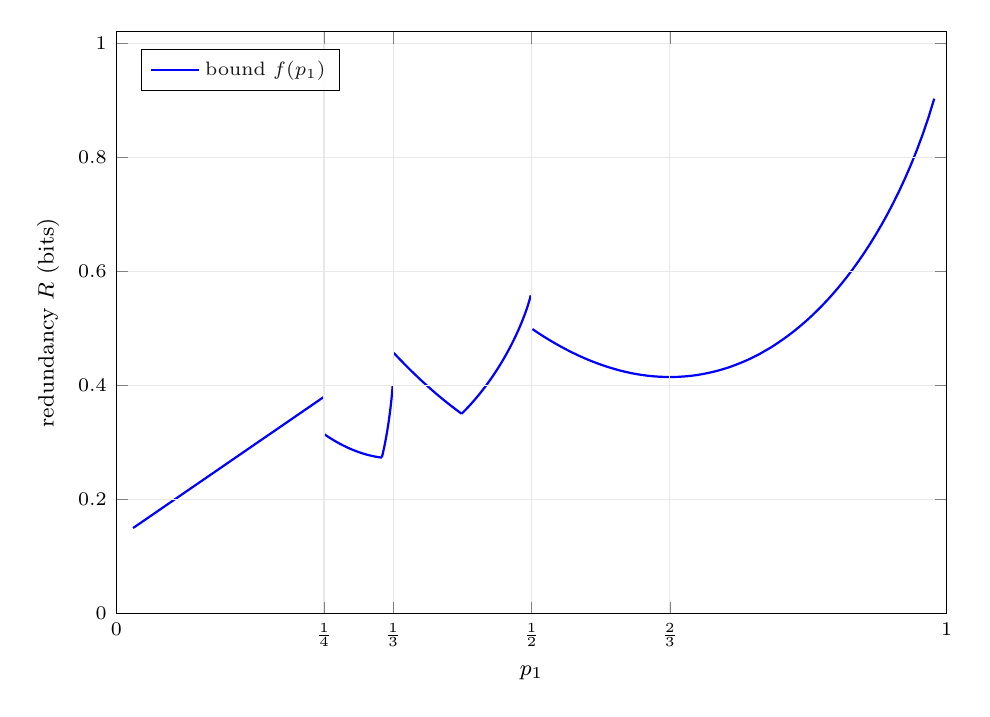
\begin{tikzpicture}
\begin{axis}[
  width=\columnwidth, height=0.74\columnwidth,
  xlabel={$p_1$}, ylabel={redundancy $R$ (bits)},
  xmin=0, xmax=1, ymin=0, ymax=1.02,
  xtick={0,0.25,0.33333,0.5,0.66667,1},
  xticklabels={$0$,$\tfrac14$,$\tfrac13$,$\tfrac12$,$\tfrac23$,$1$},
  legend pos=north west, legend cell align=left,
  legend style={font=\scriptsize,fill opacity=0.9},
  tick label style={font=\scriptsize}, label style={font=\footnotesize},
  grid=both, grid style={gray!18}, axis on top,
  declare function={
    ii(\x)=-\x*ln(\x)/ln(2);
    aff(\x)=\x+0.130119;
    pib(\x)=1.5+0.0650595-\x-ii(\x)-ii(0.5-\x);
    thb(\x)=(4+2*\x)/3+2*(1-\x)*0.565059/3-ii(\x)-ii((1-\x)/3)-ii(2*(1-\x)/3);
    nb(\x)=3-3*\x-3*ii(\x)-ii(1-3*\x);
    wib(\x)=1-ii(\x)-ii(1-\x)+(1-\x)*0.565059;
    feb(\x)=(5-\x)/3+(2-\x)*0.130119/3-ii(\x)-ii((1-2*\x)/3)-ii((2-\x)/3);
    vbb(\x)=2-\x-ii(\x)-ii(1-\x);
  }]
\addplot[blue,thick,domain=0.02:0.25,samples=50]{aff(x)};
\addlegendentry{bound $f(p_1)$}
\addplot[blue,thick,domain=0.25:0.319,samples=40]{pib(x)};
\addplot[blue,thick,domain=0.319:0.3196,samples=8]{thb(x)};
\addplot[blue,thick,domain=0.3197:0.3327,samples=30]{nb(x)};
\addplot[blue,thick,domain=0.3340:0.4158,samples=50]{wib(x)};
\addplot[blue,thick,domain=0.4158:0.499,samples=50]{feb(x)};
\addplot[blue,thick,domain=0.501:0.985,samples=70]{vbb(x)};
\end{axis}
\end{tikzpicture}
\caption{The seven-piece envelope $f(p_1)$ of Theorem~\ref{thm:main}, continuous
except for jumps at $\tfrac14$, $\tfrac13$, and $\tfrac12$. The jumps at
$\tfrac14$ and $\tfrac12$ are downward; the one at $\tfrac13$ is upward, from
$N(\tfrac13^{-})=2-\lgg3$ to
$W_{\mathrm{iso}}(\tfrac13)=2-\lgg3+\tfrac{\CC}3$. The envelope is the exact
supremum of $R$ given $p_1$ on the pieces $N$ ($[b_2,\tfrac13)$) and $V$
($[\tfrac12,1)$).}
\label{fig:envelope}
\end{figure}

The affine estimate $R<p_1+\CC$ holds on all of $p_1<\tfrac12$
(Corollary~\ref{cor:aff}), but it is active only below $\tfrac14$ in the
proposed envelope. On $[\tfrac13,\tfrac12)$ the two middle branches strictly
improve it (Proposition~\ref{prop:dom}); together they form a V-shaped curve
falling from $2-\lgg3+\CC/3$ at $\tfrac13$ to its crossing value at $p^*$ and
rising to $K$ at $\tfrac12$. On $[\tfrac14,\tfrac13)$ the three curves
$\Pi,\Theta,N$ are selected by the two crossings $b_1,b_2$
(Theorem~\ref{thm:quarter}); the structural reason is the no-burial lemma
(Lemma~\ref{lem:noburial-q}), which forces the most probable symbol to have
depth exactly two in this interval.

\begin{proposition}[Tightness]\label{prop:tight}
\begin{enumerate}
\item[\textup{(a)}] For every $p_1\in[\tfrac12,1)$,
  \[
  \begin{aligned}
    &\sup\{R(p):p\text{ a source with largest symbol }p_1\}\\
    &\qquad\qquad=2-p_1-\Hh(p_1);
  \end{aligned}
  \]
  the supremum is approached but not attained. The final branch of
  Theorem~\ref{thm:main} is therefore best possible.
\item[\textup{(b)}] $R<1$ for every source, and the supremum of $R$ over all
  sources equals $1$, i.e.\ $\sup_{p} R(p)=1$; so no constant bound smaller than
  $1$ is possible, and the branches (each $<1$, the final $\to1$ as $p_1\to1$)
  are consistent with this.
\item[\textup{(c)}] On $[b_2,\tfrac13)$ the $N$ branch is the exact
  supremum of $R$ given $p_1$, approached but not attained
  (Proposition~\ref{prop:tight-q}).
\end{enumerate}
\end{proposition}

\section{Overview of the Proof}\label{sec:outline}

We start from the universal bound $R\le 1-p_n<1$ of Kraj\v{c}i, Liu, Mike\v{s},
and Moser \cite{Krajci15} (Lemma~\ref{lem:univ}); everything else comes from the
Fano recursion (Lemma~\ref{lem:rec}). Figure~\ref{fig:dep} gives the dependency.

\emph{The affine potential.} The bound $R<p_1+\CC$ holds for all $p_1<\tfrac12$
(Corollary~\ref{cor:aff}), by strong induction on the number of symbols. It does
not close directly; it closes on the potential $\Psi=p_1+\CC-\lam\,p_n$
(Theorem~\ref{thm:aff}), where the term $-\lam p_n$ in the least symbol absorbs
the entropy of the root split. Both constants are forced: $\lam=1+5\kp(\tfrac15)$
by a balanced three-way split, and $\CC=\cthree+\tfrac{\lam-1}3$ by the uniform
ternary source, where equality holds. The only multivariate step
(Lemma~\ref{lem:B2}) is a four-parameter entropy inequality, reduced to a convex
function at the six vertices of a polytope.

\emph{The envelope.} Substituting $R<p_1+\CC$ through one more level of the
recursion sharpens the bound on $[\tfrac13,\tfrac12)$ to the V-shaped envelope
$\max(W_{\mathrm{iso}},F_\ell)$ (Theorem~\ref{thm:mid}) and gives the cap $R<K$
(Corollary~\ref{cor:kcap}).

\emph{The quarter window.} Below $\tfrac13$ the root cannot isolate the largest
symbol, but the no-burial lemma (Lemma~\ref{lem:noburial-q}) still puts it at
depth two. Substituting the whole chain proved so far back through the recursion
gives the three-piece ceiling $\max(\Pi,\Theta,N)$ on $[\tfrac14,\tfrac13)$
(Theorem~\ref{thm:quarter}), whose top piece $N$ is again exactly tight
(Proposition~\ref{prop:tight-q}).

Every scalar inequality in these substitutions has the same form, an affine
function minus an entropy of affine arguments compared to zero, and is settled
by the certification method of Appendix~\ref{app:cert}.

\begin{figure*}[t]
\centering
\footnotesize
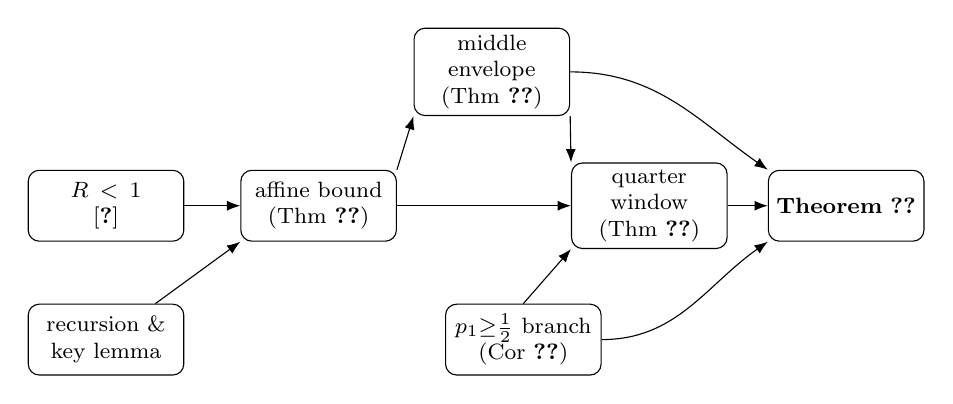
\begin{tikzpicture}[>=Latex,
  box/.style={draw,rounded corners,align=center,font=\footnotesize,
    inner sep=2.5pt, minimum height=9mm, text width=18mm}]
\node[box] (klmm) at (0,0)      {$R<1$\\ \cite{Krajci15}};
\node[box] (rec)  at (0,-1.7)   {recursion \&\\ key lemma};
\node[box] (aff)  at (2.7,0)     {affine bound\\ (Thm~\ref{thm:aff})};
\node[box] (env)  at (4.9,1.7)   {middle envelope\\ (Thm~\ref{thm:mid})};
\node[box] (quar) at (6.9,0)     {quarter window\\ (Thm~\ref{thm:quarter})};
\node[box] (half) at (5.3,-1.7)  {$p_1{\ge}\tfrac12$ branch\\ (Cor~\ref{cor:isob})};
\node[box] (main) at (9.4,0)     {\textbf{Theorem~\ref{thm:main}}};
% spine
\draw[->] (klmm) -- (aff);
\draw[->] (aff)  -- (quar);
\draw[->] (quar) -- (main.west);
% feeders from below
\draw[->] (rec)  -- (aff.south west);
\draw[->] (half.north) -- (quar.south west);
% envelope branch above the spine
\draw[->] (aff.north east) -- (env.south west);
\draw[->] (env.south east) -- (quar.north west);
% assembly into the main theorem
\draw[->] (env.east)  to[out=0,in=145] (main.north west);
\draw[->] (half.east) to[out=0,in=215] (main.south west);
\end{tikzpicture}
\caption{Logical dependency of the results. The KLMM bound starts an affine
induction; substituting it back through the recursion gives the middle envelope
and the cap $R<K$; a further substitution below $\tfrac13$ gives the
quarter-window ceiling; the pieces combine into Theorem~\ref{thm:main}.}
\label{fig:dep}
\end{figure*}

\section{Discussion}\label{sec:disc}

\begin{remark}[Where the bound is tight]\label{rem:where}
The branch $2-p_1-\Hh(p_1)$ is the exact supremum for every $p_1\ge\tfrac12$
(Proposition~\ref{prop:tight}(a)), and $R<1$ is sharp over all sources. In the
potential form (Theorem~\ref{thm:aff}) both parameters are pinned: the
coefficient $\lam=1+5\kp(\tfrac15)$ is the least the shape-$(3,3)$ argument
admits ($\sup_{0<t\le1/5}\kp(t)/t=\lam-1$ exactly,
Lemma~\ref{lem:kappa}(ii)), and, given $\lam$, the constant
$\CC=\psi(\tfrac13)=\cthree+\tfrac{\lam-1}3$ is the smallest for
which the induction closes, with equality exactly at the uniform ternary
source; the same critical value $\beta=-1-\lgg3+\tfrac{10}9\lgg5$ appears as
the maximum of Case A and as $F(W_1)$ in Case B2, at the same balanced
configuration $p_1=p_2=\tfrac13$.
\end{remark}

\begin{remark}[A simpler proof of a weaker constant]\label{rem:simple}
If one bounds the $(1,3)$ shape by the induction hypothesis alone, without
expanding the recursion a further step, the same case analysis closes with the cruder coefficient
$\tfrac65$ in place of $\lam$ (justified by the quadratic bound of
Lemma~\ref{lem:kappa}(i): in shape $(3,3)$,
$E\le(2a-1)^2\le p_k^2\le\tfrac15p_k$) and the constant
$3\cthree=5-3\lgg3=0.2451\ldots$ in place of $\CC$: the $(1,3)$ requirement
becomes $1-\Hh(p_1)\le3\cthree\,p_1$ on $[\tfrac13,\tfrac12)$, which holds by
concavity with equality at $p_1=\tfrac13$.
\end{remark}

\begin{remark}[Limits of the method]\label{rem:limits}
The affine constant $\CC$ is not the least slope-one excess. The worst sources
for $R-p_1$ are near-uniform: several equal leading symbols followed by a long
near-uniform tail, for which the redundancy splits as an algebraic term plus
(tail mass) times the redundancy of the uniform tail, whose supremum over the
tail size is the fluctuation constant $\sigma=1-\lgg e+\lgg\lgg e$ of
uniform-source redundancy. Pushing the slope-one constant to its true value
would therefore require bounding the redundancy of the near-uniform blocks in
the recursion by $\sigma$-type constants; for Huffman codes this is exactly what
the sibling property provides \cite{Gallager78}, and Fano codes lack it. All
techniques here are sibling-free. Within the present min-corrected induction the
two constants are pinned: the uniform ternary source forces
$\CC=\cthree+(\lam-1)/3$, and the shape-$(3,3)$ argument forces
$\lam-1\ge\sup_{0<t\le1/5}\kp(t)/t=5\kp(\tfrac15)$, both attained; the $(3,3)$
equality geometry ($a=\tfrac35$, three left symbols of mass $\tfrac15$) is the
four-equal-leader configuration at $p_1=\tfrac15$ against which $\lam$ is tight.
Any further improvement must break the uniform-ternary binding itself, for
instance by an exact treatment of three-symbol blocks in place of the induction
hypothesis, rather than by sharpening the scalar estimates.
\end{remark}

\appendices

\section{Structural Lemmas and the Recursion}\label{sec:tools}

\begin{lemma}[Recursion and node sum]\label{lem:rec}
If the root splits into a left part of mass $a$ and right part of mass $1-a$,
with renormalised sub-sources $B_L,B_R$, then
\[
\begin{aligned}
  R\ &=\ \bigl(1-\Hh(a)\bigr)+a\,R(B_L)+(1-a)\,R(B_R),\\
  1-\Hh(a)&=\kp(2a-1).
\end{aligned}
\]
Iterating: $R=\sum_{v}M_v\bigl(1-\Hh(a_v)\bigr)$, the sum over internal nodes
$v$, where $M_v$ is the global mass of the block at $v$ and $a_v$ is its
left-mass fraction.
\end{lemma}

\begin{proof}
Every symbol in a part is one level deeper than in the renormalised sub-source, so
$L=1+a\,L(B_L)+(1-a)\,L(B_R)$. The entropy grouping rule gives
$\mathrm H=\Hh(a)+a\,\mathrm H(B_L)+(1-a)\,\mathrm H(B_R)$. Subtract, and telescope down the tree
(leaves contribute $0$).
\end{proof}

\begin{lemma}[Chord, quadratic, and ratio bounds]\label{lem:kappa}
\begin{enumerate}
\item[\textup{(i)}] For $d\in[-1,1]$,
\[
  \kp(d)\le|d|,\qquad \kp(d)\le d^2 .
\]
\item[\textup{(ii)}] $\kp$ is strictly convex on $[-1,1]$ and strictly
increasing on $[0,1]$, and the ratio $\kp(t)/t$ is strictly increasing on
$(0,1]$; consequently
\[
\begin{aligned}
  &\kp(t)\ \le\ 5\,\kp(\tfrac15)\,t\ =\ (\lam-1)\,t
  \quad\text{on }[0,\tfrac15],\\
  &\text{with equality iff }t\in\{0,\tfrac15\},
\end{aligned}
\]
and $\lam-1=\sup_{0<t\le1/5}\kp(t)/t$ exactly.
\end{enumerate}
\end{lemma}

\begin{proof}
(i) $\kp$ is convex and even with $\kp(0)=0$ and $\kp(1)=1$. A convex function
lies below the \emph{chord} joining any two points of its graph, so on $[0,1]$
the graph of $\kp$ lies below the segment from $(0,0)$ to $(1,1)$; this gives
$\kp(d)\le(1-d)\kp(0)+d\kp(1)=d$, and evenness extends it to $\kp(d)\le|d|$. We
refer to this estimate as the \emph{chord bound}. The
quadratic bound follows from the Taylor expansion
\[
\begin{aligned}
  \Hh\Bigl(\tfrac{1+d}{2}\Bigr)\ &=\ 1-\frac{1}{\ln2}\sum_{k\ge1}\frac{d^{2k}}{2k(2k-1)},\\
  \text{i.e.}\quad
  \kp(d)\ &=\ \frac{1}{\ln2}\sum_{k\ge1}\frac{d^{2k}}{2k(2k-1)}.
\end{aligned}
\]
Since $d^{2k}\le d^2$ for $|d|\le1$ and
$\sum_{k\ge1}\tfrac1{2k(2k-1)}=\sum_{k\ge1}\bigl(\tfrac1{2k-1}-\tfrac1{2k}\bigr)
=1-\tfrac12+\tfrac13-\cdots=\ln2$ (the alternating harmonic series), it follows
that $\kp(d)\le\tfrac{d^2}{\ln2}\cdot\ln2=d^2$.

(ii) $\Hh''(x)=-\tfrac1{x(1-x)\ln2}<0$ makes $\Hh$ strictly concave, hence
$\kp$ strictly convex (affine inner map). For $0<s<t\le1$, writing
$s=\tfrac st\,t+(1-\tfrac st)\cdot0$, strict convexity and $\kp(0)=0$ give
$\kp(s)<\tfrac st\,\kp(t)$, i.e.\ $\kp(s)/s<\kp(t)/t$: the ratio is strictly
increasing, and since $\kp(t)>0$ for $t>0$ the same display shows that $\kp$
is strictly increasing on $[0,1]$. The stated bound is the ratio at
$t=\tfrac15$, using $\kp(\tfrac15)=(\lam-1)/5$, the definition
\eqref{eq:constants} of $\lam$.
\end{proof}

\begin{lemma}[Key lemma: imbalance $\le$ least left symbol]\label{lem:key}
At every internal node, the chosen split satisfies $|m_L-m_R|\le p_k$, where
$p_k$ is the last \textup{(}least\textup{)} symbol of the left part. Moreover, when
$m_L<m_R$ one has $m_R-m_L\le p_{k+1}$, the first symbol of the right part.
\end{lemma}

\begin{proof}
Let the cut be after position $k$ and $x=m_L-m_R$. If $x\ge0$ and the left part
is a singleton, then $x=2p_k-M\le p_k$ directly ($M$, the block mass, is
$\ge p_k$). Otherwise, for $x\ge0$, moving the cut one
step left transfers $p_k$ to the right and yields imbalance $|x-2p_k|$;
optimality of the cut gives $x\le|x-2p_k|$. If $x>2p_k$ this reads
$x\le x-2p_k$, impossible; hence $x\le2p_k$ and then $x\le2p_k-x$, i.e.\
$x\le p_k$. If $x<0$: were the right part a single symbol, the left part would
contain at least one symbol $\ge$ that symbol, giving $x\ge0$; so the cut can move
one step right, transferring $p_{k+1}$, and the same argument gives
$-x\le p_{k+1}\le p_k$.
\end{proof}

\begin{lemma}[Krajci--Liu--Mikes--Moser~\cite{Krajci15} universal bound]\label{lem:univ}
For the Shannon--Fano/Fano splitting code,
\[
  R\le1-p_n .
\]
In particular $R<1$ for every finite source.
\end{lemma}

\begin{lemma}[Isolation criterion and reduction]\label{lem:iso}
The root splits the leader off alone \textup{(}left part $=\{1\}$\textup{)} iff
$2p_1+p_2\ge1$; in particular this holds whenever $p_1\ge\tfrac12$, and it forces
$p_1\ge\tfrac13$. In that case
\[
\begin{aligned}
  R\ &=\ \bigl(1-\Hh(p_1)\bigr)+(1-p_1)\,R(\rho),\\
  \rho&=\tfrac{1}{1-p_1}\,(p_2,\dots,p_n).
\end{aligned}
\]
\end{lemma}

\begin{proof}
As the cut moves right the signed imbalance $2(\text{prefix mass})-1$ strictly
increases. The cut after position $1$ is at least as good as the cut after position $2$ iff
$|2p_1-1|\le|2(p_1+p_2)-1|$, which simplifies (in both sign cases) to
$2p_1+p_2\ge1$; and when this holds, the signed imbalance at position $2$ is
already $2p_1+2p_2-1\ge p_2\ge0$, so all later cuts are worse. Conversely, if
$2p_1+p_2<1$ the cut after position~$2$ is strictly better than after
position~$1$. With $p_2\le p_1$, $2p_1+p_2\ge1$ forces $3p_1\ge1$. The identity
is Lemma~\ref{lem:rec} with $a=p_1$ and $R(B_L)=0$.
\end{proof}

\begin{corollary}[Isolation ceiling]\label{cor:isob}
If $2p_1+p_2\ge1$ \textup{(}in particular if $p_1\ge\tfrac12$\textup{)}, then
$R<2-p_1-\Hh(p_1)$. More generally, for any block in which the most probable symbol is split off on its own, the
redundancy is less than $2-\beta-\Hh(\beta)$, where $\beta$ is that
symbol's fraction of the block mass.
\end{corollary}

\begin{proof}
Lemma~\ref{lem:iso} and $R(\rho)<1$ (Lemma~\ref{lem:univ}) give
$R<(1-\Hh(p_1))+(1-p_1)$; the block form is the same computation after
renormalisation.
\end{proof}

\subsection{The Tight Branch $p_1\ge\tfrac12$}\label{sec:half}

The final branch of Theorem~\ref{thm:main} is Corollary~\ref{cor:isob}. We now
prove Proposition~\ref{prop:tight}(a),(b).

\begin{proof}[Proof of Proposition~\ref{prop:tight}(a)]
The upper bound is Corollary~\ref{cor:isob}. For the lower bound fix
$p_1\in[\tfrac12,1)$ and $q\in[\tfrac12,1)$, and consider the three-symbol source
\[
  p\ =\ \bigl(p_1,\ (1-p_1)q,\ (1-p_1)(1-q)\bigr),
\]
which is sorted since $(1-p_1)q\le p_1$ for $p_1\ge\tfrac12$. Since $2p_1\ge1$
the root splits the leader off on its own (Lemma~\ref{lem:iso}), and the remaining binary block has
redundancy $1-\Hh(q)$. Hence
\[
\begin{aligned}
  R&=\bigl(1-\Hh(p_1)\bigr)+(1-p_1)\bigl(1-\Hh(q)\bigr)\\
  &\ \xrightarrow[q\to1^-]{}\ 2-p_1-\Hh(p_1).
\end{aligned}
\]
The supremum is not attained because $R<2-p_1-\Hh(p_1)$ always
(Corollary~\ref{cor:isob}).
\end{proof}

\begin{proof}[Proof of Proposition~\ref{prop:tight}(b)]
$R<1$ is Lemma~\ref{lem:univ}. For the supremum, the binary source
$(1-\varepsilon,\varepsilon)$ has $R=1-\Hh(\varepsilon)\to1$ as
$\varepsilon\to0^+$.
\end{proof}

\begin{remark}
Corollary~\ref{cor:isob} bounds $R$ by $2-p_1-\Hh(p_1)$ whenever $2p_1+p_2\ge1$,
i.e.\ also for a range of sources with $p_1\in[\tfrac13,\tfrac12)$. Only the
condition on $(p_1,p_2)$, not $p_1\ge\tfrac12$ itself, is used.
\end{remark}

\section{The Affine Potential Bound}\label{sec:affine}

The second branch follows from a stronger statement, proved by induction, in
which a multiple of the least symbol is subtracted. This correction is what makes
the induction close; since the least symbol is positive, it may be dropped at the
end, leaving the bound $R<p_1+\CC$.

\begin{theorem}[Potential form]\label{thm:aff}
For every source with $n\ge3$ symbols,
\[
  R\ \le\ \Psi(p)\ :=\ p_1+\CC-\lam\,p_n ,
\]
with equality iff $p=(\tfrac13,\tfrac13,\tfrac13)$.
\end{theorem}

\begin{corollary}\label{cor:aff}
For every source with $n\ge2$ symbols, $R<p_1+\CC$. In particular the
first \textup{(}$0<p_1<\tfrac14$\textup{)} branch of Theorem~\ref{thm:main}
holds \textup{(}$p_1<\tfrac12$ forces $n\ge3$\textup{)}.
\end{corollary}

\begin{proof}[Proof of the corollary]
For $n\ge3$, Theorem~\ref{thm:aff} gives $R\le p_1+\CC-\lam p_n<p_1+\CC$
since $\lam,p_n>0$. For $n=2$ (where necessarily $p_1\ge\tfrac12$), the chord
bound (Lemma~\ref{lem:kappa}) gives $R=\kp(2p_1-1)\le2p_1-1<p_1<p_1+\CC$.
\end{proof}

\subsection{Characterising root shapes}

The root split cuts the sorted list $p_1\ge\cdots\ge p_n$ into a left part,
which contains the leader $p_1$, and a right part. We record its
\emph{shape} as the ordered pair of these two part sizes, with any size of
three or more written simply as $3$. Thus shape $(1,2)$ means the leader
sits alone on the left with exactly two symbols on the right; $(1,3)$ means
the leader alone on the left with three or more symbols on the right; and
$(3,3)$ means at least three symbols on each side.

\begin{lemma}[Shapes]\label{lem:shapes}
Let $p_1<\tfrac12$ and $n\ge3$. Then the shape of the root split is one of
\[
  (1,2),\quad(1,3),\quad(2,2),\quad(2,3),\quad(3,3),
\]
unless the source is uniform with $n\in\{3,5\}$ \textup{(}handled separately in
\S\ref{ss:unif}\textup{)}. Moreover a split of shape $(1,\cdot)$ satisfies
$2p_1+p_2\ge1$, hence $p_1\ge\tfrac13$; a split of shape $(2,\cdot)$ or
$(3,\cdot)$ \textup{(}a \emph{group} split\textup{)} satisfies $2p_1+p_2<1$,
and the mass $a$ of its left part obeys $a<\tfrac23$; a group split of shape $(2,\cdot)$ has
$a\ge\tfrac25$.
\end{lemma}

\begin{proof}
The isolate/group dichotomy and $p_1\ge\tfrac13$ are Lemma~\ref{lem:iso}. For a
group split, $p_1\ge p_2$ gives $\tfrac32a\le\tfrac32(p_1+p_2)\le2p_1+p_2<1$,
so $a<\tfrac23$. For shape $(2,\cdot)$: if $a\ge\tfrac12$ then $a\ge\tfrac25$
trivially; if $a<\tfrac12$, Lemma~\ref{lem:key} gives $1-2a=|2a-1|\le p_2$,
while $p_2\le\tfrac a2$ (as $p_1\ge p_2$, $p_1+p_2=a$), so $1\le\tfrac52a$. It remains to exclude shapes with right part of size $1$, and shape $(3,2)$.

\textbf{Right part of size $1$} (cut after $n-1$): the imbalance is $1-2p_n$, and
Lemma~\ref{lem:key} gives $1-2p_n\le p_{n-1}\le p_1<\tfrac12$, so
$p_n>\tfrac14$. For $n\ge4$ all symbols then exceed $\tfrac14$ and the total mass
exceeds $1$, a contradiction. For $n=3$, cutting after position $1$ (imbalance
$1-2p_1$) is at least as good as after position $2$ (imbalance $1-2p_3\ge1-2p_1$),
with equality only if $p_1=p_3$, i.e.\ the uniform ternary source.

\textbf{Shape $(3,2)$} (cut after $n-2$, $n\ge5$): let $s=p_{n-1}+p_n$. If
$s\ge\tfrac12$ then $p_{n-1}\ge\tfrac s2\ge\tfrac14$, so all symbols exceed
$\tfrac14$ and again the mass exceeds $1$; hence $s<\tfrac12$ and the imbalance
is $1-2s>0$. Moving the cut one step left transfers $p_{n-2}$ and produces
signed imbalance $1-2s-2p_{n-2}$; optimality requires
$1-2s\le|1-2s-2p_{n-2}|$, which forces $1-2s-2p_{n-2}<0$ and
\begin{equation}\label{eq:32a}
  p_{n-2}+2p_{n-1}+2p_n\ \ge\ 1 .
\end{equation}
On the other hand the $n-2$ largest symbols are each $\ge p_{n-2}$, so
\begin{equation}\label{eq:32b}
  (n-2)\,p_{n-2}+p_{n-1}+p_n\ \le\ 1 .
\end{equation}
Subtracting \eqref{eq:32a} from \eqref{eq:32b}:
$(n-3)p_{n-2}\le p_{n-1}+p_n\le2p_{n-2}$, hence $n\le5$. For $n=5$ all the
inequalities are forced into equalities, giving $p_1=\cdots=p_5=\tfrac15$, the
uniform quinary source.
\end{proof}

\subsection{Scalar inequalities}

Throughout we use the standing observation that the entropy
$\mathrm H(a_1(t),\dots,a_k(t))$ of affine arguments is a concave
function of $t$ (each $\mathrm I$ is concave), so that subtractive
affine and entropy expressions are convex and are maximised at endpoints of
intervals.

\begin{lemma}\label{lem:scalar}
\begin{enumerate}
\item[\textup{(S1)}] $\psi(x):=1-\Hh(x)+(\lam-1)(1-2x)$ is strictly
decreasing on $[\tfrac13,\tfrac12]$, and
$\psi(\tfrac13)=\cthree+\tfrac{\lam-1}{3}=\CC$.
\item[\textup{(S2)}] $h(x):=\bigl(2-2x-\Hh(x)\bigr)+\tfrac{\lam-1}{2}(1-x)
\ \le\ \tfrac{\lam-1}{4}$ on $[\tfrac12,1]$, and $\tfrac{\lam-1}4<\CC$.
\item[\textup{(S3)}] \textup{(chord)} $1-\Hh(a)\ \le\ 6\cthree\,(a-\tfrac12)$ on
$[\tfrac12,\tfrac23]$.
\end{enumerate}
\end{lemma}

\begin{proof}
(S1) $\psi'(x)=-\Hh'(x)-2(\lam-1)=\lgg\tfrac{x}{1-x}-2(\lam-1)<0$ for
$x\le\tfrac12$ (the logarithm is $\le0$ there and $\lam>1$), and
$\psi(\tfrac13)=\cthree+\tfrac{\lam-1}{3}$, which is the definition
\eqref{eq:constants} of $\CC$; by \eqref{eq:cancel} the $\lgg3$-terms cancel
and $\CC=4-\tfrac53\lgg5$.

(S2) $h$ is convex ($-\Hh$ convex plus affine), so its maximum on $[\tfrac12,1]$
is at an endpoint: $h(\tfrac12)=0+\tfrac{\lam-1}{4}$ and $h(1)=0$. And
$\tfrac{\lam-1}4<\tfrac{\lam-1}2<\CC$.

(S3) $1-\Hh$ is convex, hence lies below its chord on $[\tfrac12,\tfrac23]$
through $\bigl(\tfrac12,0\bigr)$ and $\bigl(\tfrac23,1-\Hh(\tfrac23)\bigr)$;
and $\Hh(\tfrac23)=\Hh(\tfrac13)$, so the chord's slope is
$\cthree/\tfrac16=6\cthree$.
\end{proof}

\subsection{Induction}\label{ss:induct}

We prove Theorem~\ref{thm:aff} by strong induction on $n$: the full
statement (the inequality together with its equality clause) is
assumed for all sources with $3\le n'<n$ symbols (IH). In the recursion
(Lemma~\ref{lem:rec}) a part $S$ with symbols $p_i\ge\cdots\ge p_j$ and mass $w$
contributes $w\,R(B_S)$, which we bound by
\begin{equation}\label{eq:children}
  w\,R(B_S)\ \le\
  \begin{cases}
    0,\\
    \quad |S|=1,\\[2pt]
    p_i-p_j,\\
    \quad |S|=2\quad(\text{chord: }w\,\kp\bigl(\tfrac{p_i-p_j}{w}\bigr)\\
    \qquad\quad\le p_i-p_j),\\[2pt]
    p_i+w\,\CC-\lam\,p_j,\\
    \quad |S|\ge3\quad(\text{IH}),
  \end{cases}
\end{equation}
the middle bound with equality iff $p_i=p_j$ (Lemma~\ref{lem:kappa}(i);
$\tfrac{p_i-p_j}{w}=1$ is impossible as $p_j>0$), the last with equality iff
$B_S$ is uniform ternary (the IH's equality clause). Let the root split have
left mass $a$ and set $E:=1-\Hh(a)=\kp(2a-1)$. By
Lemmas~\ref{lem:kappa} and~\ref{lem:key},
\begin{equation}\label{eq:E}
  E\ \le\ |2a-1|\ \le\ p_k
  \qquad\text{and}\qquad
  E\ \le\ (2a-1)^2 ,
\end{equation}
$p_k$ being the least symbol of the left part. Writing $\Phi$ for the resulting
upper bound on $R$, it suffices in each case to show $\Phi\le\Psi
=p_1+\CC-\lam p_n$, tracking where equality can occur.

\medskip\noindent\textbf{Dominant leader ($p_1\ge\tfrac12$).}
The root splits the leader off on its own; the rest $\rho$ has $n-1\ge2$ symbols and least symbol
$\tfrac{p_n}{1-p_1}$, so Lemma~\ref{lem:univ} gives
$R\le(1-\Hh(p_1))+(1-p_1)-p_n$. Then, using $p_n\le\tfrac12(1-p_1)$ and
$\lam>1$,
\[
\begin{aligned}
  R-\Psi\ &\le\ \bigl(2-2p_1-\Hh(p_1)\bigr)+(\lam-1)p_n-\CC\\
  &\le\ h(p_1)-\CC\ \le\ \tfrac{\lam-1}{4}-\CC\ <\ 0
\end{aligned}
\]
by (S2).

\smallskip
For $p_1<\tfrac12$ we go through the shapes of Lemma~\ref{lem:shapes}. Shapes
$(1,\cdot)$ have $p_1\in[\tfrac13,\tfrac12)$; group shapes have $a<\tfrac23$.

\medskip\noindent\textbf{Shape $(1,2)$ (so $n=3$): the binding case.}
Here $\Phi=\bigl(1-\Hh(p_1)\bigr)+(p_2-p_3)$ and
\[
  \Phi-\Psi=\bigl(1-\Hh(p_1)\bigr)+p_2+(\lam-1)p_3-p_1-\CC .
\]
Substituting $p_3=1-p_1-p_2$, the middle terms equal
$(2-\lam)p_2+(\lam-1)(1-p_1)$, increasing in $p_2$ (since $\lam<2$); at
the extreme $p_2=p_1$ (so $p_3=1-2p_1$),
\[
\begin{aligned}
  \Phi-\Psi\ &\le\ \bigl(1-\Hh(p_1)\bigr)+(\lam-1)(1-2p_1)-\CC\\
  &=\ \psi(p_1)-\CC\ \le\ \psi(\tfrac13)-\CC\ =\ 0
\end{aligned}
\]
by (S1). Equality requires
$p_1=\tfrac13$ and $p_2=p_1$ (the $p_2$-coefficient $2-\lam$ is
positive) and equality in the chord bound for the right part, i.e.\
$p_2=p_3$: the uniform ternary source. This is the extremal case, and it is
what forces the value of the constant, since $\CC=\psi(\tfrac13)$ is the
smallest for which the bound can hold.

\medskip\noindent\textbf{Shape $(2,3)$.}
Here $a=p_1+p_2\in[\tfrac25,\tfrac23)$ and
$\Phi-\Psi=E+(p_1-p_2)+p_3-p_1-a\,\CC\le E-a\,\CC$ (since $p_3\le p_2$; the
$\lam p_n$-terms cancel). On
$[\tfrac25,\tfrac12]$: $E\le(2a-1)^2$ by \eqref{eq:E}, and
$\tfrac{(2a-1)^2}{a}$ has derivative of the sign of $2a-1$, hence is decreasing
there, so $\tfrac Ea\le\tfrac{(1/5)^2}{2/5}<\CC$. On
$[\tfrac12,\tfrac23)$, (S3) gives
$\tfrac Ea\le6\cthree\bigl(1-\tfrac1{2a}\bigr)<\tfrac32\cthree<\CC$. Hence
$E<a\CC$ and $\Phi<\Psi$.

\medskip\noindent\textbf{Shape $(2,2)$ (so $n=4$).}
Here $a=p_1+p_2\in[\tfrac25,\tfrac23)$ and
\[
\begin{aligned}
  \Phi-\Psi&=E+(p_1-p_2)+(p_3-p_4)-p_1-\CC+\lam p_4\\
   &=E-p_2+p_3+(\lam-1)p_4-\CC .
\end{aligned}
\]
With $p_3+p_4=1-a$ fixed,
$-p_2+p_3+(\lam-1)p_4=-p_2+(2-\lam)p_3+(\lam-1)(1-a)$
is increasing in $p_3$ ($\lam<2$), hence maximal at $p_3=p_2$, where it equals
$(\lam-1)(1-a-p_2)$; and $p_2\ge p_3\ge\tfrac{1-a}{2}$ gives
$(\lam-1)(1-a-p_2)\le\tfrac{\lam-1}{2}(1-a)$. Therefore
$\Phi-\Psi\le E+\tfrac{\lam-1}{2}(1-a)-\CC$. On $[\tfrac25,\tfrac12]$: with
$E\le(2a-1)^2$, the bound $(2a-1)^2+\tfrac{\lam-1}{2}(1-a)$ is convex with
endpoint values $\tfrac1{25}+\tfrac3{10}(\lam-1)$ at $a=\tfrac25$ and
$\tfrac{\lam-1}{4}$ at $a=\tfrac12$, and both are less than $\CC$:
$\tfrac{\lam-1}4<\CC$, while
$\tfrac1{25}+\tfrac3{10}(\lam-1)-\CC<0$. On $[\tfrac12,\tfrac23)$:
with (S3), $6\cthree(a-\tfrac12)+\tfrac{\lam-1}{2}(1-a)$ has positive slope
$6\cthree-\tfrac{\lam-1}{2}$, so on $a<\tfrac23$,
\[
  \Phi-\Psi\ <\ 6\cthree\cdot\tfrac16+\frac{\lam-1}{2}\cdot\frac13-\CC
  <\ 0. 
\]

\medskip\noindent\textbf{Shape $(3,3)$.}
Here the $\CC$-terms and $p_1,p_n$ cancel and
$\Phi-\Psi=E+p_{k+1}-\lam p_k$. The left part has at least $3$ symbols of
total mass $a$, so its least symbol obeys $p_k\le\tfrac a3$. If $a\ge\tfrac12$,
then \eqref{eq:E} gives $2a-1\le p_k\le\tfrac a3$, whence $a\le\tfrac35$ and
$p_k\le\tfrac15$; if $a<\tfrac12$ then $p_k\le\tfrac a3<\tfrac15$. In
either case $|2a-1|\le p_k\le\tfrac15$, so by Lemma~\ref{lem:kappa}(ii)
($\kp$ increasing, then the ratio bound),
\[
\begin{aligned}
  E\ &=\ \kp(2a-1)\ \le\ \kp(p_k)\ \le\ (\lam-1)\,p_k ,\\
  \text{so}\quad
  E+p_{k+1}\ &\le\ (\lam-1)p_k+p_k\ =\ \lam\,p_k ,
\end{aligned}
\]
using $p_{k+1}\le p_k$: $\Phi\le\Psi$. This case needs no constant at all,
it is what forces the correction coefficient, and by
Lemma~\ref{lem:kappa}(ii) the value $\lam=1+5\kp(\tfrac15)$ is exactly the
least coefficient this argument admits.

For strictness, suppose $R=\Psi$ in this shape; then every estimate above
is an equality. Equality in $\kp(p_k)\le(\lam-1)p_k$ with $0<p_k\le\tfrac15$
forces $p_k=\tfrac15$ (the ratio is strictly increasing); this rules
out $a<\tfrac12$ (there $p_k<\tfrac16$), so $a\ge\tfrac12$, and equality in
$\kp(|2a-1|)\le\kp(p_k)$ forces $2a-1=\tfrac15$, i.e.\ $a=\tfrac35$ ($\kp$
strictly increasing on $[0,1]$). The left part then has $\ge3$ symbols, each
$\ge p_k=\tfrac15$, of total mass $\tfrac35$: it is exactly
$(\tfrac15,\tfrac15,\tfrac15)$; also $p_{k+1}=p_k=\tfrac15$. Finally $R=\Phi$
requires equality in the right-part bound \eqref{eq:children}, and the right
part has $\ge3$ symbols, so by the equality clause of the IH its
renormalisation is uniform ternary: $p_{k+1}=\tfrac{1-a}3=\tfrac2{15}$,
contradicting $p_{k+1}=\tfrac15$. Hence $R<\Psi$, and the inequality is strict.

\subsection{Uniform case}\label{ss:unif}

These are verified for every minimising cut, so ties are immaterial.

\textbf{Uniform ternary} $(\tfrac13,\tfrac13,\tfrac13)$: either minimising cut
gives $R=1-\Hh(\tfrac13)=\cthree$, while
\[
  \Psi=\tfrac13+\CC-\tfrac{\lam}3
      =\tfrac13+\Bigl(\cthree+\frac{\lam-1}{3}\Bigr)-\frac{\lam}{3}
      =\cthree .
\]
Thus $R=\Psi$ exactly, the equality announced in Theorem~\ref{thm:aff}.

\textbf{Uniform quinary} $(\tfrac15,\dots,\tfrac15)$: either minimising cut is a
$2$--$3$ split (imbalance $\tfrac15$ both ways); the binary block has
redundancy $0$ and the ternary block is uniform ternary, so
$R=\kp(\tfrac15)+\tfrac35\,\cthree$. On the other side, since
$\tfrac{\lam}5=\tfrac15+\kp(\tfrac15)$ by \eqref{eq:constants},
$\Psi=\tfrac15+\CC-\tfrac{\lam}5=\CC-\kp(\tfrac15)$, so $\kp(\tfrac15)$
appears on both sides and, using $\CC=\cthree+\tfrac53\kp(\tfrac15)$,
\[
  \Psi-R\ =\ \CC-2\kp(\tfrac15)-\tfrac35\cthree
  \ =\ \tfrac25\,\cthree-\tfrac13\,\kp(\tfrac15)
  \ >\ 0.
\]

\subsection{The Isolate Shape $(1,3)$}\label{sec:onethree}

This case takes the most work. The root splits the leader off on its own, and the rest
$\rho=(p_2,\dots,p_n)/s$, $s=1-p_1$, has at least three symbols; write $c=p_2/s$
for its leader fraction and note $p_1\in[\tfrac13,\tfrac12)$. Applying
the induction hypothesis to $\rho$ directly gives too weak a bound; instead we
expand the recursion one step further and examine the root split of $\rho$
itself. This gives three cases, according to how $\rho$ splits.

\subsection*{Case A: $\rho$ splits its leader off on its own}

This holds in particular whenever $c\ge\tfrac12$. Write $t:=s-p_2=1-p_1-p_2$
for the mass of the tail $(p_3,\dots,p_n)$ (at least two symbols), and let $R''$
be the redundancy of that tail after renormalisation, $(p_3,\dots,p_n)/t$.
Applying Lemma~\ref{lem:rec} at the root and at $\rho$'s root, together with the
grouping identity $\Hh(p_1)+s\,\Hh(p_2/s)=\mathrm H(p_1,p_2,t)$, gives
\begin{equation}\label{eq:2level}
  R\ =\ \bigl(2-p_1-\mathrm H(p_1,p_2,t)\bigr)+t\,R'' .
\end{equation}
If that tail has $\ge3$ symbols, the
induction hypothesis gives $t\,R''\le p_3+t\CC-\lam p_n$; if it has exactly
two symbols, the chord bound gives $t\,R''\le p_3-p_n$, and then
$t\,R''+\lam p_n\le p_3+(\lam-1)p_n\le p_3+\tfrac{\lam-1}2t\le p_3+t\CC$
(using $p_n\le\tfrac t2$ and $\tfrac{\lam-1}2<\CC$). In
either case, $R\le\Psi$ reduces to $G(p_1,p_2)\le0$, where
\[
\begin{aligned}
  G(p_1,p_2)\ :=\ &2-2p_1-\mathrm H(p_1,p_2,t)+p_3-\CC\,(p_1+p_2),\\
  &\qquad p_3\le\min(p_2,t).
\end{aligned}
\]

\begin{lemma}\label{lem:caseA}
On the region
$\bigl\{\tfrac13\le p_1\le\tfrac12,\ 1-2p_1\le p_2\le p_1,\
p_3\le\min(p_2,t)\bigr\}$,
\[
  G\ \le\ \beta\ :=\ \tfrac53-\lgg3-\tfrac23\CC\ <\ 0 .
\]
\end{lemma}

\begin{proof}
$G$ is increasing in $p_3$, so put $p_3=\min(p_2,t)$; the junction is
$p_2=\tfrac{1-p_1}2$ (where $p_2=t$), which lies in $[1-2p_1,\,p_1]$ exactly for
$p_1\ge\tfrac13$. On each of the two $p_2$-segments, $G$ is
``affine $-$ entropy of affine arguments'', hence convex in $p_2$; so its
maximum is at $p_2\in\{1-2p_1,\ \tfrac{1-p_1}2,\ p_1\}$. This leaves three
one-variable functions of $p_1$, each again convex (same reason), so each is
maximised at $p_1\in\{\tfrac13,\tfrac12\}$:
\begin{itemize}
\item $p_2=1-2p_1$ (then $t=p_1$, $p_3=1-2p_1$):
  at $p_1=\tfrac13$ the value is
  $2-\tfrac23-\lgg3+\tfrac13-\tfrac23\CC=\tfrac53-\lgg3-\tfrac23\CC=\beta$;
  at $p_1=\tfrac12$ it is $1-\mathrm H(\tfrac12,0,\tfrac12)+0-\tfrac{\CC}2
  =-\tfrac{\CC}2<0$.
\item $p_2=\tfrac{1-p_1}2$ (then $p_3=t=p_2$):
  at $p_1=\tfrac13$ the value is again $\beta$ (all three symbols
  $\tfrac13$); at $p_1=\tfrac12$ it is
  $1-\mathrm H(\tfrac12,\tfrac14,\tfrac14)+\tfrac14-\tfrac34\CC
  =-\tfrac14-\tfrac34\CC<0$.
\item $p_2=p_1$ (then $p_3=1-2p_1$): this function is pointwise $\le$ the first
  one, since it has the same entropy term (by symmetry of $\mathrm H$) and the
  same $p_3$, but the larger subtraction $\CC\cdot2p_1\ge\CC\,(1-p_1)$ for
  $p_1\ge\tfrac13$.
\end{itemize}
The two $\tfrac12$-endpoint values are $\le\beta$: indeed
$-\tfrac14-\tfrac34\CC<-\tfrac{\CC}2$, and
\[
  \beta+\frac{\CC}2\ =\ \frac53-\lgg3-\frac{\CC}6\ >\ 0 .
\]
Hence $G\le\beta$ on the whole region, and $\beta<0$ by simple arithmetic.
\end{proof}

\subsection*{Case B1: $\rho$ splits as a group, $c\le\tfrac13$}

Here the induction hypothesis on $\rho$ ($\ge3$ symbols) suffices:
$s\,R(\rho)\le p_2+s\CC-\lam p_n$, so, using $p_2\le\tfrac s3$,
\[
\begin{aligned}
  R-\Psi\ &\le\ \bigl(1-\Hh(p_1)\bigr)+p_2-p_1-\CC p_1\\
  &\le\ \bigl(1-\Hh(p_1)\bigr)+\tfrac{1-p_1}3-(1+\CC)\,p_1\ =:\ b(p_1).
\end{aligned}
\]
$b'(p_1)=\lgg\tfrac{p_1}{1-p_1}-\tfrac43-\CC<0$ on $[\tfrac13,\tfrac12)$ (the
logarithm is negative), so
\[
  b\ \le\ b(\tfrac13)\ =\ \cthree-\tfrac19-\tfrac{\CC}3
  \ <\ 0.
\]


\subsection*{Case B2: $\rho$ splits as a group, $\tfrac13<c<\tfrac12$}

In absolute masses, let $\rho$ split into $L'=(p_2,\dots,p_m)$, $m\ge3$, of
mass $A$, and $R''=(p_{m+1},\dots,p_n)$ with mass $s-A$. Three preliminary
observations.

\textbf{(i) $L'$ is a dominant block.} Lemma~\ref{lem:key} applied to the block
$(p_2,\dots,p_n)$ gives $|2A-s|\le p_m$; since $c>\tfrac13$ means $s<3p_2$,
\[
  A\ \le\ \tfrac{s+p_m}2\ \le\ \tfrac{s+p_2}2\ <\ 2p_2,
\]
so $p_2/A>\tfrac12$, and within $L'$ its most probable symbol is again split off on its own. By the block
form of Corollary~\ref{cor:isob} and the grouping rule,
\[
\begin{aligned}
  &A\,R_{L'}\ \le\ 2A-p_2-A\,\Hh\bigl(\tfrac{p_2}A\bigr),\\
  &\mathrm H(p_1,A,s{-}A)+A\,\Hh\bigl(\tfrac{p_2}A\bigr)
  =\mathrm H(p_1,p_2,A{-}p_2,s{-}A)
\end{aligned}
\]
(when $|L'|=2$ the displayed bound is immediate from $R_{L'}=1-\Hh(p_2/A)$ and
$p_2\le A$).

\textbf{(ii) $R''$ is not a singleton.} If it were $\{p_n\}$, the cut after symbol
$n-1$ would have been chosen; but the cut after symbol $2$ (available since
$n-1\ge3$) has imbalance $s-2p_2\le s-2p_n$, with equality only if
$p_2=p_n$, which would make all of $p_2,\dots,p_n$ equal, forcing
$c=p_2/s=\tfrac1{n-1}\le\tfrac13$ and contradicting $c>\tfrac13$. So the cut
after symbol $2$ is strictly better, a contradiction (no tie rule is invoked). If $|R''|=2$,
the chord bound, $p_n\le\tfrac{s-A}2$ and $\tfrac{\lam-1}2<\CC$ give, as in
Case A, $(s-A)R''+\lam p_n\le p_{m+1}+(s-A)\CC$; if $|R''|\ge3$ the induction
hypothesis gives the same.

\textbf{(iii)} Combining (i) and (ii) with the two-level expansion \eqref{eq:2level}
(Lemma~\ref{lem:rec} applied at the root and at $\rho$'s root), the requirement
$R\le\Psi$ reduces to $\Delta\le0$, where
\begin{equation}\label{eq:B2}
\begin{split}
  \Delta\ :=\ &2-2p_1+2A-p_2-\mathrm H\bigl(p_1,p_2,A{-}p_2,s{-}A\bigr)\\
  &+p_{m+1}-\CC\,(p_1+A).
\end{split}
\end{equation}

\begin{lemma}[The B2 inequality]\label{lem:B2}
$\Delta\le\max\bigl(\beta,-\tfrac1{45}\bigr)<0$ for
every tuple $(p_1,p_2,A,q,r)$
\textup{(}$q=p_m$, $r=p_{m+1}$\textup{)} satisfying
\[
\begin{aligned}
  &\textup{(P1) }\tfrac13\le p_1\le\tfrac12;\quad
  \textup{(P2) }2p_1+p_2\ge1;\\
  &\textup{(P3) }\tfrac s3\le p_2\le\tfrac s2;\quad
  \textup{(P4) }0\le q\le A-p_2;
\end{aligned}
\]
\[
  \textup{(P5) }|2A-s|\le q;\qquad
  \textup{(P6) }0\le r\le q\qquad (s=1-p_1).
\]
Every case-\textup{B2} configuration satisfies \textup{(P1)--(P6)}: \textup{(P1),
(P2)} by Lemma~\ref{lem:iso}, \textup{(P3)} from $\tfrac13<c<\tfrac12$,
\textup{(P4)} because the left block $(p_2,\dots,p_m)$ has mass $A$, so $A-p_2=p_3+\cdots+p_m$ is a sum of symbols one of which is $q=p_m$ and the rest nonnegative, giving $0<q\le A-p_2$; \textup{(P5)} by
Lemma~\ref{lem:key}, \textup{(P6)} by sorting.
\end{lemma}

\begin{proof}
\textbf{Step 1 (change of variables).} Set $x=p_1$, $y=p_2$, $u=A-p_2$,
$v=s-A$; then $x+y+u+v=1$ and $x,y,u\ge0$. From (P4), (P5):
$2A-s\le q\le u$ gives $y+u-v\le u$, i.e.\ $v\ge y$; and $s-2A\le q\le u$ gives
$v\le y+2u$. In these variables, using $r\le q\le u$ (P6), (P4) and that
$\Delta$ is nondecreasing in $r$,
\[
\begin{aligned}
  \Delta\ \le\ F(x,y,u)\ &:=\ 2-2x+y+3u-\mathrm H(x,y,u,v)\\
  &\phantom{{}:={}}-\CC\,(x+y+u),\\
  &\phantom{{}:={}}v=1-x-y-u .
\end{aligned}
\]

\textbf{Step 2 (the polytope).} Conditions (P1)--(P3), together with the two consequences $v\ge y$ and $v\le y+2u$ of (P5) from Step 1,
translate to: $\tfrac13\le x\le\tfrac12$; $2x+y\ge1$; $x+3y\ge1$; $x+2y\le1$;
$x+2y+u\le1$ ($v\ge y$); $x+2y+3u\ge1$ ($v\le y+2u$). Call this polytope
$\cP$ (note $u\ge0$ is implied by the last two with $x+2y\le1$).

\textbf{Step 3 (convexity).} $F$ is affine minus
$\mathrm H(x,y,u,v)=\sum_k\mathrm I(a_k)$, a sum of the concave function
$\mathrm I$ evaluated at the affine arguments $a_k\in\{x,y,u,v\}$; hence
$-\mathrm H$, and with it $F$, is convex on $\cP$.

\textbf{Step 4 (a hull of six points).} We show that $\cP$ lies in the convex hull of the six points $W_1,\dots,W_6$, where
\[
  \begin{aligned}
  W_1&=\bigl(\tfrac13,\tfrac13,0\bigr),&
  W_2&=\bigl(\tfrac25,\tfrac15,\tfrac1{15}\bigr),&
  W_3&=\bigl(\tfrac25,\tfrac15,\tfrac15\bigr),\\
  W_4&=\bigl(\tfrac12,\tfrac16,\tfrac1{18}\bigr),&
  W_5&=\bigl(\tfrac12,\tfrac16,\tfrac16\bigr),&
  W_6&=\bigl(\tfrac12,\tfrac14,0\bigr).
  \end{aligned}
\]
The idea is to project $\cP$ onto the $(x,y)$-plane and then lift back.
Eliminating $u$, the pair $(x,y)$ ranges over the planar region
$\{\tfrac13\le x\le\tfrac12,\ y^-(x)\le y\le y^+(x)\}$ with
$y^+(x)=\tfrac{1-x}2$ and $y^-(x)=\max\bigl(1-2x,\tfrac{1-x}3\bigr)$, the two
bounds crossing at $x=\tfrac25$. This region is the quadrilateral with corners
$Q_1=(\tfrac13,\tfrac13)$, $Q_2=(\tfrac25,\tfrac15)$, $Q_3=(\tfrac12,\tfrac16)$,
$Q_4=(\tfrac12,\tfrac14)$: its upper edge $y=y^+(x)$ is the segment $Q_1Q_4$,
and its lower edge $y=y^-(x)$ is the segment $Q_1Q_2$ for $x\le\tfrac25$ and
$Q_2Q_3$ for $x\ge\tfrac25$, as the parametrisations
\[
  \bigl(x,y^+(x)\bigr)=(1-\lambda)Q_1+\lambda Q_4,\qquad \lambda=6x-2,
\]
\[
  \bigl(x,y^-(x)\bigr)=
  \begin{cases}
  (1-\lambda)Q_1+\lambda Q_2,\quad \lambda=15x-5, & x\le\tfrac25,\\
  (1-\lambda)Q_2+\lambda Q_3,\quad \lambda=10x-4, & x\ge\tfrac25,
  \end{cases}
\]
show; hence every $(x,y)$ in the region is a convex combination of
$Q_1,\dots,Q_4$. To lift back to $\cP$, fix such an $(x,y)$: the constraints
$x+2y+u\le1$ and $x+2y+3u\ge1$ confine $u$ to the interval
$\bigl[\tfrac{1-x-2y}3,\ 1-x-2y\bigr]$, whose two endpoints are affine in
$(x,y)$. Writing $u$ as a convex combination of these two endpoints, and
substituting for $(x,y)$ its expression as a convex combination of the $Q_i$,
exhibits $(x,y,u)$ as a convex combination of the six points
$\bigl(Q_i,\tfrac{1-x-2y}3\big|_{Q_i}\bigr)$ and
$\bigl(Q_i,(1-x-2y)\big|_{Q_i}\bigr)$. Since $1-x-2y$ equals
$0,\tfrac15,\tfrac16,0$ at $Q_1,\dots,Q_4$, these six points are exactly
$W_1,\dots,W_6$.

\textbf{Step 5 (certified evaluation).} By convexity,
$\max_\cP F\le\max_jF(W_j)$. Write $F=N-\mathrm H-\CC M$ with $N=2-2x+y+3u$,
$M=x+y+u$, so that $\CC M=4M-\tfrac53M\lgg5$; with
$\lgg6=1+\lgg3$, $\lgg{15}=\lgg3+\lgg5$, $\lgg{18}=1+2\lgg3$,
$\lgg\tfrac52=\lgg5-1$, $\lgg\tfrac{18}5=1+2\lgg3-\lgg5$, direct evaluation
gives
\[
\begin{array}{l}
F(W_1)=-1-\lgg3+\tfrac{10}9\lgg5=\beta,\\[3pt]
F(W_2)=-\tfrac23-\tfrac25\lgg3+\tfrac49\lgg5,\\[3pt]
F(W_3)=-\tfrac45+\tfrac13\lgg5,\\[3pt]
F(W_4)=-\tfrac{23}9-\tfrac56\lgg3+\tfrac{40}{27}\lgg5,\\[3pt]
F(W_5)=-\tfrac83-\tfrac12\lgg3+\tfrac{25}{18}\lgg5,\\[3pt]
F(W_6)=-\tfrac{13}4+\tfrac54\lgg5 .
\end{array}
\]
Each value is monotone in $\lgg3$ and in $\lgg5$ (sign of the coefficient);
substituting $\lgg3>\tfrac{19}{12}$, $\lgg5<\tfrac73$ gives
\begin{align*}
  F(W_2)&\le\tfrac{-180-171+280}{270}=-\tfrac{71}{270},\\
  F(W_3)&\le-\tfrac45+\tfrac13\cdot\tfrac73=-\tfrac1{45},\\
  F(W_4)&\le\tfrac{-1656-855+2240}{648}=-\tfrac{271}{648},\\
  F(W_5)&\le\tfrac{-576-171+700}{216}=-\tfrac{47}{216},\\
  F(W_6)&\le-\tfrac{13}4+\tfrac{35}{12}=-\tfrac13,
\end{align*}
so $F(W_j)\le-\tfrac1{45}$ for $j=2,\dots,6$; and $F(W_1)=\beta<0$, critical at the same
balanced configuration $p_1=p_2=\tfrac13$ as in Case~A. Hence
$\Delta\le F\le\max\bigl(\beta,-\tfrac1{45}\bigr)<0$ on $\cP$.
\end{proof}

\begin{remark}
Both constraint families in Lemma~\ref{lem:B2} are essential: dropping
isolation (P2) admits
$(p_1,p_2,A,q,r)=(\tfrac13,\tfrac29,\tfrac49,\tfrac29,\tfrac29)$ with
$\Delta=\tfrac{26}9-\tfrac53\lgg3-\tfrac79\CC>0$, and dropping
the split constraint
(P5) admits $(\tfrac13,\tfrac13,\tfrac23,\tfrac13,\tfrac13)$ with
$\Delta=\tfrac83-\lgg3-\CC>0$.
The Shannon--Fano optimality of the cut is thus the
mechanism that makes \eqref{eq:B2} true, entering the proof only through its
two linear consequences $y\le v\le y+2u$.
\end{remark}

\medskip
Cases A, B1, B2 exhaust shape $(1,3)$ (if $\rho$ does not isolate its leader
then $c<\tfrac12$), each with strict inequality, so, together with
\S\ref{ss:induct}--\ref{ss:unif}, the induction closes; every case is strict:
the dominant case, shapes $(2,3)$, $(2,2)$, $(3,3)$ (the latter via the
equality clause of the IH), the three cases of shape $(1,3)$, and the uniform
quinary source, except shape $(1,2)$, which is tight exactly at the
uniform ternary source, where equality indeed holds (\S\ref{ss:unif}).
Theorem~\ref{thm:aff}, and with it the affine branch of
Theorem~\ref{thm:main}, are proved; the middle branches are the topic of
the next section. \qed

\section{The Middle Envelope on $[\tfrac13,\tfrac12)$}\label{sec:midcap}

Substituting the affine bound back into the recursion yields the two middle
branches of Theorem~\ref{thm:main}: a non-affine, V-shaped envelope on $[\tfrac13,\tfrac12)$ that strictly improves the affine
bound on the whole interval, and hence a uniform cap for all $p_1<\tfrac12$.
Throughout this section
\[
\begin{aligned}
  K\ &:=\ \tfrac52-\tfrac56\lgg5\ =\ \tfrac{1+\CC}{2}\ =\ 0.565059\ldots,\\
  \delta\ &:=\ 1-2p_1,\qquad V(q)\ :=\ 2-q-\Hh(q),
\end{aligned}
\]
$V$ is the tight bound of
Corollary~\ref{cor:isob} for a block whose leader fraction is $q\ge\tfrac12$
(convex, since $-\Hh$ is convex). The auxiliary single curve
\[
  \tilde B(p_1)\ :=\ 1+(1+\CC)\,p_1-\Hh(p_1)
  \qquad\bigl(\tfrac13\le p_1\le\tfrac12\bigr)
\]
will lie above all the comparison curves at once; the two branches of the
envelope itself are introduced after Lemma~\ref{lem:midcomp}.
Two exact values anchor our bounds: since $\Hh(\tfrac13)=\lgg3-\tfrac23$,
\[
\begin{aligned}
  \tilde B(\tfrac13)\ &=\ 2-\lgg3+\tfrac{\CC}{3}\ =\ 0.458410\ldots,\\
  \tilde B(\tfrac12)\ &=\ \tfrac{1+\CC}{2}\ =\ K\ \ \text{exactly};
\end{aligned}
\]
and $\tilde B$ is strictly increasing on $[\tfrac13,\tfrac12]$:
\begin{equation}\label{eq:btmono}
  \tilde B'(x)\ =\ 1+\CC-\lgg\tfrac{1-x}{x}\ \ge\ 1+\CC-\lgg2\ =\ \CC\ >\ 0,
\end{equation}
because $\tfrac{1-x}{x}\le2$ for $x\ge\tfrac13$. Everything rests on a fine
description of the \emph{group} case (the root does not isolate the leader),
where the leader has depth two.

\begin{lemma}[Fine group bounds]\label{lem:fine}
Let $\tfrac13\le p_1<\tfrac12$ and let the root split be a group split
($2p_1+p_2<1$) with left mass $a$; put $x:=a-p_1>0$ and, for $0<x<1-p_1$,
\[
\begin{aligned}
  F(p_1,x)\ &:=\ 1+p_1+2x+(1-p_1-x)\,\CC\\
  &\phantom{{}:={}}-\mathrm H\bigl(p_1,x,1-p_1-x\bigr),\\
  G(p_1,x)\ &:=\ F(p_1,x)+x\,\CC .
\end{aligned}
\]
If the left part has exactly two symbols, then $R<F(p_1,x)$ and
$x\in[\tfrac\delta3,\delta]$; if it has at least three, then $R<G(p_1,x)$ and
$x\in[\tfrac{2\delta}5,\tfrac{2\delta}3]$. Consequently
\[
  R\ <\ \max\Bigl\{F\bigl(p_1,\tfrac\delta3\bigr),\ F(p_1,\delta),\
  G\bigl(p_1,\tfrac{2\delta}5\bigr),\ G\bigl(p_1,\tfrac{2\delta}3\bigr)\Bigr\}.
\]
\end{lemma}

\begin{proof}
The left part has at least two symbols: its leader is $p_1$, and its remainder
$L'$ has mass $x$, largest symbol $p_2$ and least symbol $p_k$ ($k$ is the cut
position), so $p_k\le x$. Lemma~\ref{lem:key} at the root reads
$|2a-1|=|2x-\delta|\le p_k$. Since $|2x-\delta|\le x$ gives $x\le\delta$,
i.e.\ $a\le1-p_1\le2p_1$ (as $p_1\ge\tfrac13$), the leader's fraction of the
left part is $p_1/a\ge\tfrac12$, so the leader is again split off on its own within the left part
(Lemma~\ref{lem:iso}); this reduction applied inside the left part and the
grouping identity
$(1-\Hh(a))+a\bigl(1-\Hh(p_1/a)\bigr)=(1+a)-\mathrm H(p_1,x,1-a)$ give
\[
  R=(1+a)-\mathrm H(p_1,x,1-a)+x\,R_{L'}+(1-a)\,R_{\mathrm{Rt}},
\]
where $R_{L'}$ and $R_{\mathrm{Rt}}$ are the redundancies of the renormalised left remainder $L'$ (mass $x$) and right part $\mathrm{Rt}$ (mass $1-a$, largest symbol $p_{k+1}$). By
Corollary~\ref{cor:aff} (every source),
$(1-a)R_{\mathrm{Rt}}<p_{k+1}+(1-a)\CC$ (or $=0$ for a singleton, when the
same bound holds trivially).

\textbf{Two left symbols.} Then $L'=\{p_2\}$, so $x=p_2=p_k$ and $xR_{L'}=0$;
with $p_{k+1}\le p_k=x$,
\[
  R\ <\ (1+a)-\mathrm H(p_1,x,1-a)+x+(1-a)\,\CC\ =\ F(p_1,x),
\]
and $|2x-\delta|\le p_k=x$ reads $x\ge\tfrac\delta3$
\textup{(}$\delta-2x\le x$\textup{)} and $x\le\delta$
\textup{(}$2x-\delta\le x$\textup{)}.

\textbf{At least three left symbols.} Then $|L'|\ge2$ and $xR_{L'}<p_2+x\CC$
(Corollary~\ref{cor:aff} again); since $p_2$ and $p_k$ are distinct symbols of
$L'$, $p_2+p_{k+1}\le p_2+p_k\le x$, whence $R<F(p_1,x)+x\CC=G(p_1,x)$.
Moreover $p_k\le\min(p_2,\,x-p_2)\le\tfrac x2$, so $|2x-\delta|\le\tfrac x2$:
$x\ge\tfrac{2\delta}5$ and $x\le\tfrac{2\delta}3$.

For the endpoints, in $x$, with $t:=1-p_1-x$ and $\mathrm I'(t)=-\lgg t-\lgg e$,
\[
  \frac{\partial F}{\partial x}\ =\ 2-\CC+\lgg\frac{x}{t},
  \qquad
  \frac{\partial G}{\partial x}\ =\ 2+\lgg\frac{x}{t},
\]
both strictly increasing in $x$ ($x$ increases, $t$ decreases); so
$F(p_1,\cdot)$ and $G(p_1,\cdot)$ are decreasing-then-increasing and each is
maximised over its $x$-interval at an endpoint.
\end{proof}

\begin{lemma}[Comparisons]\label{lem:midcomp}
Write $W_{\mathrm{iso}}(p_1):=\bigl(1-\Hh(p_1)\bigr)+(1-p_1)K$ and
$T_0(x):=3-3x-2\mathrm I(x)-\mathrm I(1-2x)$; by the grouping identity,
$T_0(x)=(1-\Hh(x))+(1-x)V\bigl(\tfrac{x}{1-x}\bigr)$. On
$[\tfrac13,\tfrac12]$, with $\delta=1-2p_1$:
\begin{enumerate}
\item[\textup{(o)}] $\tfrac13+\CC<K$:
  $\ K-\tfrac13-\CC=\tfrac56\lgg5-\tfrac{11}6>0$.
\item[\textup{(i)}] $W_{\mathrm{iso}}\le\tilde B$, by pure algebra: since
  $K=\tfrac{1+\CC}2$, the $\Hh$-terms cancel and
  \[
  \begin{aligned}
    \tilde B(p_1)-W_{\mathrm{iso}}(p_1)\ &=\ (1+\CC)\,p_1-(1-p_1)\,\frac{1+\CC}{2}\\
    &=\ \frac{(1+\CC)(3p_1-1)}{2}\ \ge\ 0 .
  \end{aligned}
  \]
\item[\textup{(ii)}] $T_0\le\tilde B$: the difference
  $\tilde B-T_0=-2+(4+\CC)\,p_1+\mathrm I(p_1)-\mathrm I(1-p_1)+\mathrm I(\delta)$ is
  concave, with endpoint values $\tfrac{\CC}3>0$ at $\tfrac13$ and
  $\tfrac{\CC}2>0$ at $\tfrac12$.
\item[\textup{(iii)}] $F(\cdot,\delta)\le\tilde B$: since $1-p_1-\delta=p_1$,
  $F(p_1,\delta)=T_0(p_1)+\CC\,p_1$, and
  \[
    \tilde B-F(\cdot,\delta)\ =\ -2+4p_1+\mathrm I(p_1)-\mathrm I(1-p_1)+\mathrm I(\delta)
  \]
  is concave and vanishes at both endpoints: $\tilde B$ is exactly the
  concave curve pinned to the worst two-left-symbol bound at $p_1=\tfrac13$ and
  at $p_1=\tfrac12$.
\item[\textup{(iv)}] $F(\cdot,\tfrac\delta3)\le\tilde B$: the difference is
  concave with endpoint values
  $-\tfrac49+\tfrac23\lgg3-\tfrac5{27}\lgg5>0$ at $\tfrac13$
  and $0$ at $\tfrac12$.
\item[\textup{(v)}] $G(\cdot,\tfrac{2\delta}5)\le\tilde B$: the difference is
  concave with endpoint values $-\tfrac83+\tfrac{11}9\lgg5>0$
  at $\tfrac13$ and $0$ at $\tfrac12$.
\item[\textup{(vi)}] $G(\cdot,\tfrac{2\delta}3)\le\tilde B$: the difference is
  concave with endpoint values
  $-\tfrac{20}9+\tfrac23\lgg3+\tfrac59\lgg5>0$ at $\tfrac13$
  and $0$ at $\tfrac12$.
\end{enumerate}
In \textup{(ii)}--\textup{(vi)}, concavity places each difference above the
smaller endpoint value on all of $[\tfrac13,\tfrac12]$, hence $\ge0$ there.
\end{lemma}

\begin{proof}
In each of (ii)--(vi) the difference of the two curves is concave (a sum of
$\pm\mathrm I$ of affine arguments), so nonnegativity on $[\tfrac13,\tfrac12]$
follows from its two endpoint values; (o) and (i) are direct algebra.
\textbf{Concavity in
(ii)--(vi).} Each difference is affine plus terms $\pm \mathrm I(u(p_1))$ with $u$
affine of slope $s$, contributing $\pm s^2I''(u)=\mp\tfrac{s^2}{u\ln2}$ to
the second derivative; collecting them, the second derivatives times $\ln2$
are
\[
  \textup{(ii),(iii)}:\ -\tfrac1{p_1}-\tfrac4\delta+\tfrac1{1-p_1};\qquad
  \textup{(iv)}:\ -\tfrac4{3\delta}-\tfrac1{3(2-p_1)}+\tfrac1{1-p_1};
\]
\[
  \textup{(v)}:\ -\tfrac8{5\delta}-\tfrac1{5(3-p_1)}+\tfrac1{1-p_1};\qquad
  \textup{(vi)}:\ -\tfrac8{3\delta}-\tfrac1{3(1+p_1)}+\tfrac1{1-p_1},
\]
each negative: on $[\tfrac13,\tfrac12)$ one has $\tfrac1{1-p_1}\le2$, while
$\delta\le\tfrac13$ gives $\tfrac4\delta\ge12$, $\tfrac4{3\delta}\ge4$,
$\tfrac8{5\delta}\ge\tfrac{24}5$, $\tfrac8{3\delta}\ge8$, all $>2$.

\textbf{Endpoints at $\tfrac12$.} There $\delta=0$ and all four constrained
curves degenerate to
$F(\tfrac12,0)=G(\tfrac12,0)=\tfrac32+\tfrac{\CC}2-\Hh(\tfrac12)=K
=\tilde B(\tfrac12)$, while $T_0(\tfrac12)=\tfrac12=\tilde B(\tfrac12)
-\tfrac{\CC}2$: the values claimed.

\textbf{Endpoints at $\tfrac13$}, where $\delta=\tfrac13$ and
$\tilde B(\tfrac13)=\tfrac{10}3-\lgg3-\tfrac59\lgg5$ (substitute
$\CC=4-\tfrac53\lgg5$). For (ii):
$T_0(\tfrac13)=2-3\mathrm I(\tfrac13)=2-\lgg3$, so $\tilde
B(\tfrac13)-T_0(\tfrac13)=\tfrac{\CC}3$. For (iii): using
$\mathrm I(\tfrac13)=\tfrac{\lgg3}3$ and $\mathrm I(\tfrac23)=\tfrac23(\lgg3-1)$,
\[
\begin{aligned}
  &-2+\tfrac43+\mathrm I\bigl(\tfrac13\bigr)-\mathrm I\bigl(\tfrac23\bigr)
  +\mathrm I\bigl(\tfrac13\bigr)\\
  &\quad=\ -\tfrac23+\tfrac{\lgg3}3-\tfrac23(\lgg3-1)+\tfrac{\lgg3}3\ =\ 0 .
\end{aligned}
\]
For (iv)--(vi), evaluating $\mathrm H$ at the argument triples
$\bigl(\tfrac13,\tfrac19,\tfrac59\bigr)$,
$\bigl(\tfrac13,\tfrac2{15},\tfrac8{15}\bigr)$,
$\bigl(\tfrac13,\tfrac29,\tfrac49\bigr)$ and subtracting from
$\tilde B(\tfrac13)$ yields the closed forms in (iv)--(vi), each positive.
\end{proof}

The two branches of the envelope are the isolate curve $W_{\mathrm{iso}}$ of
Lemma~\ref{lem:midcomp} and the two-left-symbol endpoint curve at
$x=\tfrac\delta3$, whose explicit form (substitute $x=\tfrac\delta3$,
$1-p_1-x=\tfrac{2-p_1}3$ in Lemma~\ref{lem:fine}) is
\[
  F\bigl(p_1,\tfrac\delta3\bigr)
  \ =\ \frac{5-p_1}{3}+\frac{2-p_1}{3}\,\CC
  -\mathrm H\Bigl(p_1,\frac{1-2p_1}{3},\frac{2-p_1}{3}\Bigr).
\]
These are exactly the two middle rows of Theorem~\ref{thm:main}. One decreases and
the other increases, so they cross exactly once, as the next lemma records.

\begin{lemma}[Crossing]\label{lem:cross}
On $[\tfrac13,\tfrac12]$:
\begin{enumerate}
\item[\textup{(a)}] $W_{\mathrm{iso}}$ is strictly decreasing, with
  $W_{\mathrm{iso}}'=\lgg\tfrac{p_1}{1-p_1}-K\le-K$; and $F(\cdot,\tfrac\delta3)$
  is strictly increasing, with slope at least
  $\tfrac{9\lgg3+2\lgg5-15}{9}\ge\tfrac{77}{180}$.
\item[\textup{(b)}] $\bigl(W_{\mathrm{iso}}-F(\cdot,\tfrac\delta3)\bigr)(\tfrac13)
  =-\tfrac49+\tfrac23\lgg3-\tfrac5{27}\lgg5>0$ and
  $\bigl(W_{\mathrm{iso}}-F(\cdot,\tfrac\delta3)\bigr)(\tfrac12)=-\tfrac K2<0$;
  hence there is a unique $p^*$ with
  $W_{\mathrm{iso}}(p^*)=F\bigl(p^*,\tfrac{\delta(p^*)}3\bigr)$, and
  $F(\cdot,\tfrac\delta3)\le W_{\mathrm{iso}}$ on $[\tfrac13,p^*]$,
  $W_{\mathrm{iso}}\le F(\cdot,\tfrac\delta3)$ on $[p^*,\tfrac12]$. Numerically
  $p^*=0.415798\ldots$, with common value $0.350664\ldots$
\item[\textup{(c)}] $\tfrac25<p^*<\tfrac7{16}$:
\[
  \bigl(W_{\mathrm{iso}}-F(\cdot,\tfrac\delta3)\bigr)\bigl(\tfrac25\bigr)
  =-\tfrac{83}{30}+\tfrac65\lgg3+\tfrac7{18}\lgg5\ >\ 0,
\]
\[
\begin{aligned}
  &\bigl(F(\cdot,\tfrac\delta3)-W_{\mathrm{iso}}\bigr)\bigl(\tfrac7{16}\bigr)\\
  &\quad=\tfrac{119}{96}-\tfrac{27}{16}\lgg3+\tfrac{185}{288}\lgg5\ >\ 0 .
\end{aligned}
\]
\end{enumerate}
\end{lemma}

\begin{proof}
The single difference $W_{\mathrm{iso}}-F(\cdot,\tfrac\delta3)$ is strictly
decreasing by (a), so its unique sign change and its signs at the interior
points $\tfrac25,\tfrac7{16}$ follow from the closed-form values below.
(a) $p_1\le1-p_1$ gives the first claim. Differentiating
$F(p_1,\tfrac\delta3)$ in $p_1$ (the $\lgg e$-terms cancel, since the argument
slopes $1,-\tfrac23,-\tfrac13$ sum to zero):
\[
\begin{aligned}
  \tfrac{d}{dp_1}F\bigl(p_1,\tfrac\delta3\bigr)
  \ &=\ -\tfrac{1+\CC}{3}+\lgg3+\lgg p_1\\
  &\quad-\tfrac23\lgg\delta-\tfrac13\lgg(2-p_1)\\
  \ &\ge\ -\tfrac{1+\CC}{3}+\lgg3-\tfrac{\lgg5}3 \\
  \ &=\ \tfrac{9\lgg3+2\lgg5-15}{9},
\end{aligned}
\]
using $\lgg p_1\ge-\lgg3$, $\lgg\delta\le-\lgg3$, $\lgg(2-p_1)\le\lgg5-\lgg3$
and $\CC=4-\tfrac53\lgg5$; and $9\lgg3+2\lgg5>15$.

(b) The value at $\tfrac13$ is the endpoint value of
Lemma~\ref{lem:midcomp}(iv), since $W_{\mathrm{iso}}(\tfrac13)
=\tilde B(\tfrac13)$ by item (i) there; at $\tfrac12$,
$W_{\mathrm{iso}}(\tfrac12)=\tfrac K2$ while $F(\tfrac12,0)=K$. The
difference is strictly decreasing by (a), whence the unique zero and the sign
pattern.

(c) At $\tfrac25$ ($\delta=\tfrac15$): $\Hh(\tfrac25)
=\lgg5-\tfrac25-\tfrac35\lgg3$ gives $W_{\mathrm{iso}}(\tfrac25)
=\tfrac{29}{10}+\tfrac35\lgg3-\tfrac32\lgg5$, and
$\mathrm I(\tfrac1{15})=\tfrac1{15}(\lgg3+\lgg5)$,
$\mathrm I(\tfrac8{15})=\tfrac8{15}(\lgg3+\lgg5-3)$ give
$F(\tfrac25,\tfrac1{15})=\tfrac{17}3-\tfrac35\lgg3-\tfrac{17}9\lgg5$. At $\tfrac7{16}$ ($\delta=\tfrac18$): the terms
$\mathrm I(\tfrac7{16})$ cancel in the difference, which needs only
$\mathrm I(\tfrac1{24})=\tfrac1{24}(3+\lgg3)$,
$\mathrm I(\tfrac{25}{48})=\tfrac{25}{48}(4+\lgg3-2\lgg5)$ and
$\mathrm I(\tfrac9{16})=\tfrac9{16}(4-2\lgg3)$.
\end{proof}

\begin{lemma}[Per-piece domination]\label{lem:envdom}
Write $h:=W_{\mathrm{iso}}-F(\cdot,\delta)$ and, for a comparison curve $X$,
$e_X:=F(\cdot,\tfrac\delta3)-X$. On $[\tfrac13,\tfrac12]$:
\begin{enumerate}
\item[\textup{(i)}] $h$ is concave, $h(\tfrac13)=0$ exactly, and
\[
  h\bigl(\tfrac7{16}\bigr)
  =-\tfrac{37}{32}+\tfrac98\lgg3+\tfrac{25}{96}\lgg5-\tfrac7{16}\lgg7\ >\ 0 .
\]
Hence $F(\cdot,\delta)\le W_{\mathrm{iso}}$
on $[\tfrac13,\tfrac7{16}]\supseteq[\tfrac13,p^*]$, and
$T_0=F(\cdot,\delta)-\CC\,p_1\le W_{\mathrm{iso}}$ there as well.
\item[\textup{(ii)}] $e_{F(\cdot,\delta)}$ is concave, vanishes at $\tfrac12$,
and $e_{F(\cdot,\delta)}(p^*)=h(p^*)\ge0$ by the crossing identity
$F(p^*,\tfrac{\delta}3)=W_{\mathrm{iso}}(p^*)$ and (i); hence
$F(\cdot,\delta)\le F(\cdot,\tfrac\delta3)$ on $[p^*,\tfrac12]$.
\item[\textup{(iii)}] $e_{G(\cdot,2\delta/5)}$, $e_{G(\cdot,2\delta/3)}$ and
$e_{T_0}$ are concave, with values $0$, $0$, $\tfrac{\CC}2$ at $\tfrac12$ and,
at $\tfrac25$,
\begin{multline*}
  e_{G(\cdot,2\delta/5)}\bigl(\tfrac25\bigr)
  =\tfrac{92}{75}-\tfrac35\lgg3+\tfrac{32}{45}\lgg5-\tfrac{13}{25}\lgg13\\
  \ \ge\ -\tfrac{61}{75}-\tfrac{186}{175}\lgg3+\tfrac{1696}{1575}\lgg5
  \ >\ 0,
\end{multline*}
where the first lower bound is the chord bound
$\mathrm I(\tfrac{13}{25})\ge\tfrac57\,\mathrm I(\tfrac{64}{125})
+\tfrac27\,\mathrm I(\tfrac{27}{50})$ ($\mathrm I$ is concave and
$\tfrac{13}{25}=\tfrac57\cdot\tfrac{64}{125}+\tfrac27\cdot\tfrac{27}{50}$),
which eliminates $\lgg13$, and the second is elementary; and
\begin{gather*}
  e_{G(\cdot,2\delta/3)}\bigl(\tfrac25\bigr)
  =\tfrac{16}{15}+\tfrac19\lgg5-\tfrac7{15}\lgg7>0,\\
  e_{T_0}\bigl(\tfrac25\bigr)
  =\tfrac{46}{15}-\tfrac35\lgg3-\tfrac89\lgg5>0 .
\end{gather*}
Hence $G(\cdot,\tfrac{2\delta}5)$,
$G(\cdot,\tfrac{2\delta}3)$, $T_0\le F(\cdot,\tfrac\delta3)$ on
$[\tfrac25,\tfrac12]\supseteq[p^*,\tfrac12]$.
\item[\textup{(iv)}] $W_{\mathrm{iso}}-G(\cdot,\tfrac{2\delta}5)$ and
$W_{\mathrm{iso}}-G(\cdot,\tfrac{2\delta}3)$ are concave, positive at
$\tfrac13$ (the endpoint values of
Lemma~\ref{lem:midcomp}(v),(vi), since
$W_{\mathrm{iso}}(\tfrac13)=\tilde B(\tfrac13)$), and positive at $\tfrac25$,
where each equals the certified sum
$\bigl(W_{\mathrm{iso}}-F(\cdot,\tfrac\delta3)\bigr)(\tfrac25)+e_G(\tfrac25)$
of Lemma~\ref{lem:cross}(c) and item (iii). Hence both $G$-curves are
$\le W_{\mathrm{iso}}$ on $[\tfrac13,\tfrac25]$; and on $[\tfrac25,p^*]$ as
well, via $G\le F(\cdot,\tfrac\delta3)\le W_{\mathrm{iso}}$ (item (iii) and
Lemma~\ref{lem:cross}(b),(c)).
\end{enumerate}
Consequently every curve considered ($W_{\mathrm{iso}}$, $T_0$,
$F(\cdot,\tfrac\delta3)$, $F(\cdot,\delta)$, $G(\cdot,\tfrac{2\delta}5)$,
$G(\cdot,\tfrac{2\delta}3)$) is $\le W_{\mathrm{iso}}$ on $[\tfrac13,p^*]$
and $\le F(\cdot,\tfrac\delta3)$ on $[p^*,\tfrac12)$.
\end{lemma}

\begin{proof}
Every comparison below is between two curves whose difference is concave, so
its sign on the relevant subinterval is fixed by the closed-form values at the
endpoints $\tfrac13,\tfrac25,\tfrac7{16},\tfrac12$ computed here.
For concavity, as in Lemma~\ref{lem:midcomp}, each difference is affine
plus terms $\pm \mathrm I(u(p_1))$ with $u$ affine of slope $s$, contributing
$\mp\tfrac{s^2}{u\ln2}$ to the second derivative. Since $W_{\mathrm{iso}}$
and $\tilde B$ differ by an affine function
(Lemma~\ref{lem:midcomp}(i)), the differences in (i) and (iv) have the same
second derivatives as in Lemma~\ref{lem:midcomp}(iii),(v),(vi), and are
therefore concave. For
the differences against $F(\cdot,\tfrac\delta3)$, the second derivatives
times $\ln2$ are
\[
\begin{aligned}
  &\text{(ii), }e_{T_0}:\ -\tfrac1{p_1}-\tfrac8{3\delta}+\tfrac1{3(2-p_1)};\\
  &e_{G(\cdot,2\delta/5)}:\
  -\tfrac4{15\delta}+\tfrac{9-2p_1}{15(2-p_1)(3-p_1)};\\
  &e_{G(\cdot,2\delta/3)}:\
  -\tfrac4{3\delta}-\tfrac{\delta}{3(2-p_1)(1+p_1)},
\end{aligned}
\]
all negative on $[\tfrac13,\tfrac12)$: $\tfrac1{3(2-p_1)}\le\tfrac29<
\tfrac8{3\delta}$, and $\tfrac{9-2p_1}{15(2-p_1)(3-p_1)}
\le\tfrac{25/3}{15\cdot\frac32\cdot\frac52}=\tfrac4{27}
<\tfrac45\le\tfrac4{15\delta}$ (as $\delta\le\tfrac13$).

\textbf{Exact values.} $h(\tfrac13)=0$: both $W_{\mathrm{iso}}$ and
$F(\cdot,\delta)$ equal $\tilde B$ at $\tfrac13$
(Lemma~\ref{lem:midcomp}(i),(iii)). At $\tfrac12$: $\delta=0$ and
$F(\tfrac12,0)=G(\tfrac12,0)=K$, $T_0(\tfrac12)=K-\tfrac{\CC}2$ (proof of
Lemma~\ref{lem:midcomp}), giving the values in (ii),(iii). For
$h(\tfrac7{16})$: with $\mathrm I(\tfrac7{16})=\tfrac7{16}(4-\lgg7)$,
$\mathrm I(\tfrac9{16})=\tfrac9{16}(4-2\lgg3)$, $\mathrm I(\tfrac18)=\tfrac38$, one gets
$W_{\mathrm{iso}}(\tfrac7{16})=-\tfrac{51}{32}+\tfrac98\lgg3
-\tfrac{15}{32}\lgg5+\tfrac7{16}\lgg7$ and
$F(\tfrac7{16},\tfrac18)=-\tfrac7{16}-\tfrac{35}{48}\lgg5
+\tfrac78\lgg7$.

At $\tfrac25$ ($\delta=\tfrac15$), with
$F(\tfrac25,\tfrac1{15})=\tfrac{17}3-\tfrac35\lgg3-\tfrac{17}9\lgg5$
(Lemma~\ref{lem:cross}):
\[
\begin{aligned}
  G\bigl(\tfrac25,\tfrac2{25}\bigr)
  &=\tfrac{111}{25}-\tfrac{13}5\lgg5+\tfrac{13}{25}\lgg13,\\
  G\bigl(\tfrac25,\tfrac2{15}\bigr)
  &=\tfrac{23}5-\tfrac35\lgg3-2\lgg5+\tfrac7{15}\lgg7,
\end{aligned}
\]
\[
  T_0\bigl(\tfrac25\bigr)=\tfrac{13}5-\lgg5,
\]
and subtracting each from $F(\tfrac25,\tfrac1{15})$ gives the three stated
closed forms. For the chord bound, substitute
$\mathrm I(\tfrac{13}{25})=\tfrac{13}{25}\cdot2\lgg5-\tfrac{13}{25}\lgg13$ and
then $\mathrm I(\tfrac{64}{125})=\tfrac{64}{125}(3\lgg5-6)$,
$\mathrm I(\tfrac{27}{50})=\tfrac{27}{50}(1+2\lgg5-3\lgg3)$.
\end{proof}

\begin{theorem}[Middle envelope]\label{thm:mid}
For every source with $\tfrac13\le p_1<\tfrac12$,
\[
  R\ <\ \begin{cases}
  \,W_{\mathrm{iso}}(p_1)\ =\ 1-\Hh(p_1)+(1-p_1)\,\dfrac{1+\CC}2,\\
  \qquad \tfrac13\le p_1\le p^*,\\[8pt]
  \,F\bigl(p_1,\tfrac\delta3\bigr)\ =\ \dfrac{5-p_1}{3}
    +\dfrac{2-p_1}{3}\,\CC\\
  \qquad -\mathrm H\Bigl(p_1,\dfrac{1-2p_1}{3},\dfrac{2-p_1}{3}\Bigr),\\
  \qquad p^*\le p_1<\tfrac12.
  \end{cases}
\]
\end{theorem}

\begin{proof}
Write $E(p_1)$ for the right-hand side (well defined: the two curves agree at
$p^*$). Strong induction on $n$; a source with $p_1<\tfrac12$ has $n\ge3$,
and a block with maximal fraction in $[\tfrac13,\tfrac12)$ has at least three
symbols, so the induction is well founded. A sub-block with maximal fraction
$q$ is bounded by: $q+\CC$ if $q<\tfrac13$ (Corollary~\ref{cor:aff});
$E(q)<K$ if $q\in[\tfrac13,\tfrac12)$ (induction hypothesis, then the
monotonicity of the pieces, Lemma~\ref{lem:cross}(a): on the left piece
$E(q)\le W_{\mathrm{iso}}(\tfrac13)=2-\lgg3+\tfrac{\CC}3<K$, since
$K-W_{\mathrm{iso}}(\tfrac13)=\lgg3-\tfrac56-\tfrac5{18}\lgg5\ge\tfrac{11}{108}>0$
\textup{(}by $\lgg3>\tfrac{19}{12}$, $\lgg5<\tfrac73$\textup{)}, and on the right piece
$E(q)<F(\tfrac12,0)=K$); $V(q)$ if $q\ge\tfrac12$
(Corollary~\ref{cor:isob}). So, exactly as before, every sub-block with
maximal fraction $q<\tfrac12$ has redundancy $<K$.

\textbf{Isolate root} ($2p_1+p_2\ge1$): here $R=(1-\Hh(p_1))+(1-p_1)R(\rho)$
with leader fraction $q=p_2/(1-p_1)\le y:=p_1/(1-p_1)$, and
$y\in[\tfrac12,1)$. If $q<\tfrac13$, then $R(\rho)<\tfrac13+\CC<K$ by
Lemma~\ref{lem:midcomp}(o); if $q\in[\tfrac13,\tfrac12)$, then $R(\rho)<K$.
In both cases $R<(1-\Hh(p_1))+(1-p_1)K=W_{\mathrm{iso}}(p_1)$. If $q\ge\tfrac12$, then
$R(\rho)<V(q)\le\max\bigl(V(\tfrac12),V(y)\bigr)=\max\bigl(\tfrac12,V(y)\bigr)$,
since $V$ is convex on $[\tfrac12,y]\ni q$. If the maximum is $\tfrac12$,
then $R<(1-\Hh(p_1))+\tfrac{1-p_1}2<W_{\mathrm{iso}}$ (as $\tfrac12<K$);
otherwise $R<(1-\Hh(p_1))+(1-p_1)V(y)=T_0(p_1)$ by the grouping identity of
Lemma~\ref{lem:midcomp}. So the isolate root yields $R<W_{\mathrm{iso}}(p_1)$
or $R<T_0(p_1)$.

\textbf{Group root} ($2p_1+p_2<1$): Lemma~\ref{lem:fine} bounds $R$ strictly by
one of the four endpoint curves $F(p_1,\tfrac\delta3)$, $F(p_1,\delta)$,
$G(p_1,\tfrac{2\delta}5)$, $G(p_1,\tfrac{2\delta}3)$.

In every case $R$ is strictly below one of the six curves of
Lemma~\ref{lem:envdom}, and that lemma bounds each of them by
$W_{\mathrm{iso}}(p_1)$ on $[\tfrac13,p^*]$ and by $F(p_1,\tfrac\delta3)$ on
$[p^*,\tfrac12)$, i.e.\ by $E(p_1)$.
\end{proof}

\begin{corollary}[Single formula]\label{cor:bt}
For every source with $\tfrac13\le p_1<\tfrac12$,
\[
  R\ <\ \tilde B(p_1)\ =\ 1+(1+\CC)\,p_1-\Hh(p_1);
\]
indeed the envelope of Theorem~\ref{thm:mid} lies below $\tilde B$ pointwise,
strictly except at $p_1=\tfrac13$ and (in the limit) $p_1=\tfrac12$.
\end{corollary}

\begin{proof}
$W_{\mathrm{iso}}\le\tilde B$ is Lemma~\ref{lem:midcomp}(i), with equality
only at $\tfrac13$; $F(\cdot,\tfrac\delta3)\le\tilde B$ is
Lemma~\ref{lem:midcomp}(iv), with equality only at $\tfrac12$ (the difference
is concave, positive at $\tfrac13$, zero at $\tfrac12$).
\end{proof}

\begin{corollary}[Flat cap]\label{cor:kcap}
For every source with $p_1<\tfrac12$,
$\ R<K=\tfrac52-\tfrac56\lgg5=0.565059\ldots$
\end{corollary}

\begin{proof}
For $p_1<\tfrac13$: $R<p_1+\CC<\tfrac13+\CC<K$ by
Lemma~\ref{lem:midcomp}(o). For $p_1\in[\tfrac13,p^*]$:
$R<W_{\mathrm{iso}}(p_1)\le W_{\mathrm{iso}}(\tfrac13)
=2-\lgg3+\tfrac{\CC}3<K$, by the monotonicity of
Lemma~\ref{lem:cross}(a) and the $\tfrac{11}{108}$-certificate in the proof
of Theorem~\ref{thm:mid}. For $p_1\in[p^*,\tfrac12)$:
$R<F(p_1,\tfrac\delta3)<F(\tfrac12,0)=K$, again by
Lemma~\ref{lem:cross}(a).
\end{proof}

\begin{proposition}[Domination]\label{prop:dom}
On $[\tfrac13,\tfrac12)$ the envelope of Theorem~\ref{thm:mid} is strictly
below $p_1+\CC$: the middle branches of Theorem~\ref{thm:main} improve the
affine bound wherever both apply. Quantitatively, the margin is at least
$\tfrac23\CC-\cthree=1+\lgg3-\tfrac{10}9\lgg5=0.005042\ldots$ on the left
piece and at least $\tfrac{\CC}2=0.0650\ldots$ on the right piece.
\end{proposition}

\begin{proof}
\textbf{Left piece.} $p_1+\CC-W_{\mathrm{iso}}(p_1)$ has derivative
$1-W_{\mathrm{iso}}'=1+\lgg\tfrac{1-p_1}{p_1}+K>0$, so on $[\tfrac13,p^*]$ it
is minimised at $\tfrac13$, where (since
$W_{\mathrm{iso}}(\tfrac13)=\tilde B(\tfrac13)$) it equals
$\tfrac23\CC-\cthree=-\beta$, the critical margin of Lemma~\ref{lem:caseA}
resurfacing.

\textbf{Right piece.} $p_1+\CC-F(p_1,\tfrac\delta3)$ is concave (its second
derivative times $\ln2$ is $-\tfrac1{p_1}-\tfrac4{3\delta}
-\tfrac1{3(2-p_1)}<0$), so on $[\tfrac25,\tfrac12]\supseteq[p^*,\tfrac12)$ it
is minimised at an endpoint. At $\tfrac12$ it equals $\tfrac{\CC}2$, and at
$\tfrac25$ it equals $-\tfrac{19}{15}+\tfrac35\lgg3+\tfrac29\lgg5$, which
exceeds $\tfrac{\CC}2$; so the margin is at least $\tfrac{\CC}2$ throughout.
\end{proof}

\begin{remark}\label{rem:midquality}
The envelope decreases strictly from $2-\lgg3+\tfrac{\CC}3=0.4584\ldots$ at
$\tfrac13$ to $0.350664\ldots$ at $p^*=0.415798\ldots$, then rises strictly
to $K=0.5651\ldots$ at $\tfrac12$, so the cap needs nothing beyond the
monotonicity of the two pieces; and by Proposition~\ref{prop:dom} no minimum
with the affine bound is ever active. Against the single curve of
Corollary~\ref{cor:bt} the envelope gains $(1+\CC)\tfrac{3p_1-1}2$ on the
left piece, up to $0.1398$ at $p^*$. Every improvement of the affine constant
$\CC$ halves into $K$.
\end{remark}

\section{The Quarter-Window Ceiling on $[\tfrac14,\tfrac13)$}\label{sec:quarter}

Below $\tfrac13$ the isolate root disappears ($2p_1+p_2\le3p_1<1$). We now
apply everything proved so far, i.e., the affine bound
(Corollary~\ref{cor:aff}), the envelope (Theorem~\ref{thm:mid}) and the
$p_1\ge\tfrac12$ branch (Corollary~\ref{cor:isob}), within the recursion on
$\tfrac14\le p_1<\tfrac13$. Throughout this section $\delta:=1-2p_1$,
$K=\tfrac{1+\CC}2$ and $V(q)=2-q-\Hh(q)$ are as in
Appendix~\ref{sec:midcap}, $W_{\mathrm{iso}}$ and $F(p_1,x)$ are the
envelope ingredients of Lemmas~\ref{lem:midcomp} and~\ref{lem:fine}
(the formula for $F$ makes sense for all $0<p_1<\tfrac12$, $0<x<1-p_1$,
and is so used below), and
\[
\begin{aligned}
  F_\ell(q)\ &:=\ F\bigl(q,\tfrac{1-2q}3\bigr)\\
  &\ =\ \frac{5-q}{3}+\frac{2-q}{3}\,\CC
  -\mathrm H\Bigl(q,\frac{1-2q}{3},\frac{2-q}{3}\Bigr)
\end{aligned}
\]
is the increasing piece of the envelope
$E=\max(W_{\mathrm{iso}},F_\ell)$. The three curves of the quarter-window ceiling
are
\begin{align*}
  \Pi(p_1)&:=\tfrac32+\tfrac{\CC}2-p_1-\mathrm I(p_1)-\mathrm I\bigl(\tfrac12-p_1\bigr),\\
  \Theta(p_1)&:=\tfrac{4+2p_1}{3}+\tfrac{2(1-p_1)}{3}\,K
   -\mathrm H\Bigl(p_1,\tfrac{1-p_1}{3},\tfrac{2(1-p_1)}{3}\Bigr),\\
  N(p_1)&:=3-3p_1-3\mathrm I(p_1)-\mathrm I(1-3p_1)\\
   &\ =\ 3-3p_1-\mathrm H\bigl(p_1,p_1,p_1,1-3p_1\bigr).
\end{align*}
We use repeatedly that a sum of an affine function and terms
$-\mathrm I(u(\cdot))$ with $u$ affine is convex (each term contributes
$+c^2/(u\ln2)$ to the second derivative, where $c$ is the slope of $u$) and attains
its maximum over an interval at an endpoint.

Every sub-block is bounded using the results above: a block of absolute mass $m$
whose largest symbol is the fraction $q$ of $m$ contributes less than
$m\,\mathrm{ch}(q)$ to $R$ (and exactly $0$ if a singleton), where
\begin{equation}\label{eq:charge-q}
  \mathrm{ch}(q)\;:=\;
  \begin{cases}
    q+\CC,\\
    \quad 0<q<\tfrac13
      \quad\text{(Corollary~\ref{cor:aff})},\\[2pt]
    E(q)=\max\bigl(W_{\mathrm{iso}}(q),\,F_\ell(q)\bigr),\\
    \quad \tfrac13\le q<\tfrac12
      \quad\text{(Theorem~\ref{thm:mid})},\\[2pt]
    V(q),\\
    \quad \tfrac12\le q<1
      \quad\text{(Corollary~\ref{cor:isob})}.
  \end{cases}
\end{equation}

\begin{lemma}[Exact values]\label{lem:exact-q}
With $N_K(p_1):=1+2p_1-2\mathrm I(p_1)-\mathrm I(\delta)+\delta K$:
\[
\begin{aligned}
  &\Pi\bigl(\tfrac14\bigr)=\tfrac14+\tfrac{\CC}2,\qquad
  N\bigl(\tfrac14\bigr)=\tfrac14,\\
  &\Theta\bigl(\tfrac14\bigr)=N_K\bigl(\tfrac14\bigr)=\tfrac{1+\CC}4,
\end{aligned}
\]
\[
\begin{aligned}
  \Pi\bigl(\tfrac13\bigr)&=F\bigl(\tfrac13,\tfrac16\bigr)=1+\tfrac{\CC-\lgg3}2,\\
  \Theta\bigl(\tfrac13\bigr)&=F\bigl(\tfrac13,\tfrac19\bigr)
  =\tfrac{34}9-\tfrac53\lgg3-\tfrac{10}{27}\lgg5,
\end{aligned}
\]
\[
  F_\ell\bigl(\tfrac12\bigr)=F\bigl(\tfrac12,0\bigr)=K,\qquad
  \Theta-F\bigl(\cdot,\tfrac{1-\cdot}4\bigr)\ \text{is affine in }p_1 .
\]
\end{lemma}

\begin{proof}
Every entropy term is of the form
$\mathrm I(a/b)=\tfrac ab\bigl(\lgg b-\lgg a\bigr)$, so each value is a
rational combination of logarithms of small integers. For example, at
$p_1=\tfrac13$,
$\Theta(\tfrac13)=\tfrac{4+2/3}{3}+\tfrac{4}{9}K-\mathrm H\bigl(\tfrac13,\tfrac29,\tfrac49\bigr)$
with
$\mathrm H\bigl(\tfrac13,\tfrac29,\tfrac49\bigr)
=\tfrac{\lgg3}3+\tfrac29\bigl(\lgg9-\lgg2\bigr)+\tfrac49\bigl(\lgg9-\lgg4\bigr)
=\tfrac53\lgg3-\tfrac{10}9$; substituting $K=\tfrac52-\tfrac56\lgg5$ gives
$\Theta(\tfrac13)=\tfrac{34}9-\tfrac53\lgg3-\tfrac{10}{27}\lgg5$. The
remaining values are identical routine evaluations.
\end{proof}

\begin{lemma}[Certificates]\label{lem:cert-q}
Let $E_1,E_2,\Lambda_1,\Lambda_2,\Theta',\Theta''$ be the corner curves of
Propositions~\textup{\ref{prop:L2-q}}--\textup{\ref{prop:L3-q}} below.
The following exact signed evaluations hold on the endpoints used in the
corner reductions:
\begin{enumerate}
\item[\textup{(A1)}] $(\Pi-\Theta)(\tfrac13)
  =-\tfrac79+\tfrac76\lgg3-\tfrac{25}{54}\lgg5<0$.
\item[\textup{(A2)}] $(\Theta-N)(\tfrac13)
  =\tfrac{16}9-\tfrac23\lgg3-\tfrac{10}{27}\lgg5<0$.
\item[\textup{(A3)}] $(2-\lgg3)-\Pi(\tfrac14)
  =\tfrac56\lgg5-\lgg3-\tfrac14>0$, and
  $\tfrac13+\CC-(2-\lgg3)=\tfrac73+\lgg3-\tfrac53\lgg5>0$.
\item[\textup{(B1)}] $\tfrac13+\CC-F_\ell(\tfrac13)
  =\tfrac59+\tfrac53\lgg3-\tfrac{35}{27}\lgg5>0$.
\item[\textup{(C1)}] $\bigl(\Theta-F(\cdot,\tfrac\delta3)\bigr)(\tfrac14)
  =-\tfrac56+\tfrac34\lgg3+\tfrac59\lgg5-\tfrac7{12}\lgg7>0$.
\item[\textup{(C2)}] $\bigl(\Theta-F(\cdot,\tfrac{1-\cdot}4)\bigr)(\tfrac14)
  =\tfrac78-\tfrac{21}{16}\lgg3+\tfrac{25}{48}\lgg5>0$;\quad
  $\bigl(\Theta-F(\cdot,\tfrac{1-\cdot}4)\bigr)(\tfrac13)
  =\tfrac79-\tfrac76\lgg3+\tfrac{25}{54}\lgg5>0$.
\item[\textup{(C3)}] $(\Theta-N_K)(\tfrac13)
  =\tfrac{23}{18}-\tfrac23\lgg3-\tfrac5{54}\lgg5>0$.
\item[\textup{(D1)}] $\Pi(\tfrac13)-E_1(\tfrac14)
  =\tfrac{17}{20}-\tfrac12\lgg3+\tfrac56\lgg5-\tfrac{11}{20}\lgg{11}>0$;\quad
  $\Pi(\tfrac13)-E_1(\tfrac13)
  =-\tfrac{12}5+\tfrac12\lgg3+\tfrac{13}{18}\lgg5>0$.
\item[\textup{(D2)}] $\Pi(\tfrac13)-E_2(\tfrac14)
  =\tfrac{11}{12}+\tfrac14\lgg3-\tfrac59\lgg5>0$;\quad
  $\Pi(\tfrac13)-E_2(\tfrac13)
  =-\tfrac{14}9+\tfrac76\lgg3-\tfrac5{54}\lgg5>0$.
\item[\textup{(D3)}] $\Pi(\tfrac13)-\Lambda_1(\tfrac14)
  =\tfrac5{28}-\tfrac54\lgg3-\tfrac5{42}\lgg5+\tfrac34\lgg7>0$;\quad
  $\Pi(\tfrac13)-\Lambda_1(\tfrac13)
  =-\tfrac{26}{21}+\tfrac5{14}\lgg3+\tfrac5{18}\lgg5+\tfrac23\lgg7
  -\tfrac{11}{21}\lgg{11}>0$.
\item[\textup{(D4)}] $\Pi(\tfrac13)-\Theta''(\tfrac14)
  =\tfrac5{36}+\lgg3+\tfrac{25}{108}\lgg5-\tfrac{19}{36}\lgg{19}>0$;\quad
  $\Pi(\tfrac13)-\Theta''(\tfrac13)
  =-\tfrac{16}9+\tfrac{11}6\lgg3+\tfrac{25}{162}\lgg5-\tfrac{14}{27}\lgg7>0$.
\item[\textup{(D5)}] $(\Pi-\Lambda_2)(\tfrac14)
  =-\tfrac45-\tfrac65\lgg3+\tfrac76\lgg5>0$;\quad
  $(\Pi-\Lambda_2)(\tfrac13)
  =-\tfrac43+\tfrac3{10}\lgg3+\tfrac{17}{18}\lgg5-\tfrac7{15}\lgg7>0$.
\item[\textup{(D6)}] $(\Pi-\Theta')(\tfrac14)
  =-\tfrac{11}{14}+\tfrac5{28}\lgg5+\tfrac34\lgg7-\tfrac{13}{28}\lgg{13}>0$;\quad
  $(\Pi-\Theta')(\tfrac13)
  =-\tfrac{38}{21}+\tfrac12\lgg3-\tfrac5{14}\lgg5+\tfrac23\lgg7>0$.
\item[\textup{(S)}] $(\Theta-\Pi)(\tfrac{23}{72})
  =-\tfrac{167}{108}-\tfrac{121}{72}\lgg3+\tfrac{295}{648}\lgg5
  +\tfrac{49}{36}\lgg7-\tfrac{13}{72}\lgg{13}>0$ and
  $(\Theta-N)(\tfrac{23}{72})
  =\tfrac{59}{54}-\tfrac{13}{18}\lgg3-\tfrac{245}{648}\lgg5
  +\tfrac{49}{36}\lgg7-\tfrac{23}{36}\lgg{23}>0$.
\end{enumerate}
\end{lemma}

\begin{proof}
As in Lemma~\ref{lem:exact-q}, each item is the evaluation of the stated
curves at a rational point, hence a rational combination of
$\lgg3,\lgg5,\lgg7,\lgg{11},\lgg{13},\lgg{19},\lgg{23}$; the displayed
closed forms follow by collecting coefficients. For example, \textup{(A1)}
is $(\Pi-\Theta)(\tfrac13)$ with both values taken from
Lemma~\ref{lem:exact-q}:
$1+\tfrac{\CC-\lgg3}2-\tfrac{34}9+\tfrac53\lgg3+\tfrac{10}{27}\lgg5
=-\tfrac79+\tfrac76\lgg3-\tfrac{25}{54}\lgg5$. Each sign then follows from
Lemma~\ref{lem:certify}\textup{(i)}: replacing each $\lgg m$ by a rational
bound from its continued-fraction expansion reduces the sign to a comparison of
integer powers. Coarse bounds such as $\tfrac{19}{12}<\lgg3<\tfrac{27}{17}$
suffice for the items with a comfortable margin; the near-degenerate ones,
\textup{(A1)}, \textup{(A2)}, \textup{(C2)}, and \textup{(S)}, use
correspondingly higher convergents \textup{(}for instance
$\lgg3<\tfrac{485}{306}$, i.e.\ $3^{306}<2^{485}$\textup{)}.
\end{proof}

\begin{lemma}[Right-part bound]\label{lem:msup-q}
Let $Q\in(0,1)$. Then $\sup_{0<q\le Q}\mathrm{ch}(q)\le M(Q)$, where
\[
  M(Q)\ :=\
  \begin{cases}
    Q+\CC, & Q<\tfrac13,\\[2pt]
    \max\bigl(\tfrac13+\CC,\;F_\ell(Q)\bigr), & \tfrac13\le Q<\tfrac12,\\[2pt]
    \max\bigl(K,\;V(Q)\bigr), & \tfrac12\le Q<1 ,
  \end{cases}
\]
and $M(Q)\le Q+\CC$ for all $Q<\tfrac12$.
\end{lemma}

\begin{proof}
On $(0,\tfrac13)$ the bound $q+\CC$ increases to the limit
$\tfrac13+\CC$. On $[\tfrac13,\tfrac12)$, $E=\max(W_{\mathrm{iso}},F_\ell)$
with $W_{\mathrm{iso}}$ decreasing and $F_\ell$ increasing
(Lemma~\ref{lem:cross}(a)), so
$E(q)\le\max\bigl(W_{\mathrm{iso}}(\tfrac13),F_\ell(Q)\bigr)$ for
$q\le Q$; and $W_{\mathrm{iso}}(\tfrac13)\le\tfrac13+\CC$ is
$\tfrac32\cthree\le\CC$. On $[\tfrac12,1)$,
$V$ is convex, so
$V(q)\le\max\bigl(V(\tfrac12),V(Q)\bigr)=\max\bigl(\tfrac12,V(Q)\bigr)$,
while the $[\tfrac13,\tfrac12)$ part contributes at most
$\max(\tfrac13+\CC,K)=K$ \textup{(}Lemma~\ref{lem:midcomp}(o)\textup{)},
and $\tfrac12<K$. For the last claim it remains to check
$F_\ell(Q)\le Q+\CC$ on $[\tfrac13,\tfrac12)$: the difference
$Q+\CC-F_\ell(Q)$ is concave \textup{(}$F_\ell$ is affine plus $-\mathrm I$ of
affine arguments, hence convex\textup{)}, so it is bounded below by the
smaller of its endpoint values $\tfrac13+\CC-F_\ell(\tfrac13)>0$
\textup{(}certificate \textup{(B1)}\textup{)} and
$\tfrac12+\CC-K=\tfrac{\CC}2>0$.
\end{proof}

\begin{lemma}[No burial on $[\tfrac14,\tfrac13)$]\label{lem:noburial-q}
Let $\tfrac14\le p_1<\tfrac13$. Then:
\begin{enumerate}
\item[\textup{(i)}] the root is a group split: the left part
$L=\{p_1,\dots,p_k\}$ has $k\ge2$ symbols; write $a$ for its mass,
$x:=a-p_1>0$, $p_k$ for its least symbol, and $s:=|1-2a|$, so that
$s\le p_k$ by Lemma~\ref{lem:key};
\item[\textup{(ii)}] the left part splits its leader off by itself: $2p_1+p_2\ge a$;
hence $\ell_1=2$ exactly, and
\begin{equation}\label{eq:master-q}
  R\;=\;(1+a)-\mathrm H(p_1,x,1-a)\;+\;x\,R_{L'}\;+\;(1-a)\,R_{B},
\end{equation}
where $L'=L\setminus\{p_1\}$ \textup{(}mass $x$, largest symbol $p_2$, least
symbol $p_k$\textup{)} and $B$ is the right part \textup{(}mass $1-a$,
largest symbol $p_{k+1}\le p_k$\textup{)};
\item[\textup{(iii)}] the right part has at least two symbols.
\end{enumerate}
\end{lemma}

\begin{proof}
(i) $2p_1+p_2\le3p_1<1$, so the root does not isolate the leader
(Lemma~\ref{lem:iso}); thus $k\ge2$, and the leader lies in $L$ since
blocks are prefixes.

(ii) Suppose $2p_1+p_2<a$, i.e.\ $p_2<a-2p_1$. By Lemma~\ref{lem:key},
$s\le p_k\le p_2<a-2p_1$. If $a\le\tfrac12$ then $1-2a<a-2p_1$ gives
$a>\tfrac{1+2p_1}3\ge\tfrac12$ (using $p_1\ge\tfrac14$), a contradiction;
if $a>\tfrac12$ then $2a-1<a-2p_1$ gives $a<1-2p_1\le\tfrac12$, again a
contradiction. Hence $2p_1+p_2\ge a$ and, by Lemma~\ref{lem:iso} applied
inside $L$, $L$ splits as $\{p_1\}\,|\,L'$: the leader is a leaf at depth
$2$. Identity \eqref{eq:master-q} is the recursion (Lemma~\ref{lem:rec})
at the root, the isolate reduction inside $L$, and the grouping identity
$(1-\Hh(a))+a\bigl(1-\Hh(p_1/a)\bigr)=(1+a)-\mathrm H(p_1,x,1-a)$, exactly
as in Lemma~\ref{lem:fine}.

(iii) If $B=\{p_n\}$ then $1-a=p_n\le p_k\le p_1$, so $a\ge1-p_1>\tfrac12$;
the bound $s\le p_k$ forces $p_k\ge2a-1\ge1-2p_1$, and $p_k\le p_1$ then
gives $p_1\ge\tfrac13$, a contradiction.
\end{proof}

Both children in \eqref{eq:master-q} are now bounded by
\eqref{eq:charge-q} and Lemma~\ref{lem:msup-q} \textup{(}the right part
only through $p_{k+1}\le p_k$:
$(1-a)R_B<(1-a)\,M\bigl(p_k/(1-a)\bigr)$\textup{)}; what remains is the
coupled supremum over the constraint set of Lemma~\ref{lem:noburial-q},
organised by the size of $L'$. Write
$J(a):=(1+a)-\mathrm H(p_1,\,a-p_1,\,1-a)\ge0$ for the two-level toll in
\eqref{eq:master-q} and $Q(a):=x/(1-a)$, strictly increasing in $a$, with
$J'(a)=1+\lgg Q(a)$; the corner curves are ($N_K$ as in
Lemma~\ref{lem:exact-q}; in $\Lambda_1,\Lambda_2,\Theta',\Theta''$ the
toll $J$ is evaluated at the indicated left mass, with $x=a-p_1$ equal to
$\tfrac{3\delta}7,\tfrac{3\delta}5,\tfrac{4\delta}7,\tfrac{4\delta}9$
respectively):
\begin{align*}
  E_1(p_1)&:=2-p_1+\tfrac{3-p_1}{5}\,\CC-\mathrm I(p_1)\\
   &\phantom{{}:={}}-\mathrm I\Bigl(\tfrac{3-p_1}{5}\Bigr)-2\mathrm I\Bigl(\tfrac{1-2p_1}{5}\Bigr),\\
  E_2(p_1)&:=\tfrac{5-p_1}{3}+\tfrac{2-4p_1}{3}+\tfrac{1-2p_1}{3}
   +\tfrac{1+p_1}{3}\,\CC\\
   &\phantom{{}:={}}-\mathrm I(p_1)-\mathrm I\Bigl(\tfrac{1+p_1}{3}\Bigr)-2\mathrm I\Bigl(\tfrac{1-2p_1}{3}\Bigr),\\
  \Lambda_1(p_1)&:=J\Bigl(\tfrac{3+p_1}{7}\Bigr)+\tfrac{2\delta}{7}+(1-p_1)\,\CC,\\
  \Lambda_2(p_1)&:=J\Bigl(\tfrac{3-p_1}{5}\Bigr)+\tfrac{2\delta}{5}+(1-p_1)\,\CC,\\
  \Theta'(p_1)&:=J\Bigl(\tfrac{4-p_1}{7}\Bigr)+\tfrac{4\delta}{7}\,K\\
   &\phantom{{}:={}}+\tfrac{\delta}{7}+\tfrac{3+p_1}{7}\,\CC,\\
  \Theta''(p_1)&:=J\Bigl(\tfrac{4+p_1}{9}\Bigr)+\tfrac{4\delta}{9}\,K\\
   &\phantom{{}:={}}+\tfrac{\delta}{9}+\tfrac{5-p_1}{9}\,\CC .
\end{align*}

\begin{proposition}[$|L'|=1$]\label{prop:L1-q}
If the left part has exactly two symbols, then
\[
\begin{aligned}
  R\;<\;\max\Bigl\{&F\bigl(p_1,\tfrac{\delta}{3}\bigr),\;
  F\bigl(p_1,\tfrac{1-p_1}{4}\bigr),\;\Theta(p_1),\\
  &N_K(p_1),\;N(p_1)\Bigr\}.
\end{aligned}
\]
\end{proposition}

\begin{proof}
Here $x=p_2=p_k\le p_1$ and $R_{L'}=0$, so by \eqref{eq:master-q} and
Lemma~\ref{lem:msup-q}, $R<h(a):=J(a)+(1-a)\,M(Q(a))$. The constraint
$s\le x$ reads $a\in[\tfrac{1+p_1}3,\,1-p_1]$, and $x\le p_1$ caps
$a\le2p_1$; since $p_1\ge\tfrac14>\tfrac15$ the window is
$[\tfrac{1+p_1}3,\,2p_1]$. Along it $Q$ increases from
$\delta/(2-p_1)<\tfrac13$ \textup{(}as $p_1>\tfrac15$\textup{)} through
$Q=\tfrac13$ at $a_{13}:=\tfrac{1+3p_1}4$ and $Q=\tfrac12$ at
$a_{12}:=\tfrac{1+2p_1}3$, to $Q(2p_1)=p_1/\delta\ge\tfrac12$
\textup{(}as $p_1\ge\tfrac14$; also $a_{13}\le a_{12}\le 2p_1$
there\textup{)}.

\textbf{On $[\tfrac{1+p_1}3,a_{13}]$} ($Q\le\tfrac13$):
$h(a)=J(a)+x+(1-a)\CC=F(p_1,x)$ with $x\in[\tfrac\delta3,\tfrac{1-p_1}4]$.
Since $\partial_xF=2-\CC+\lgg\tfrac{x}{1-p_1-x}$ is strictly increasing in
$x$ (Lemma~\ref{lem:fine}), $F$ is decreasing-then-increasing, so
$h\le\max\bigl(F(p_1,\tfrac\delta3),F(p_1,\tfrac{1-p_1}4)\bigr)$.

\textbf{On $[a_{13},a_{12}]$} ($\tfrac13\le Q\le\tfrac12$):
$h\le\max\bigl(\mathrm{fl}(a),\mathrm{co}(a)\bigr)$ pointwise, where
$\mathrm{fl}(a):=J(a)+(1-a)(\tfrac13+\CC)$ and
$\mathrm{co}(a):=J(a)+(1-a)F_\ell(Q(a))$. Since
$J'=1+\lgg Q\le1+\lgg\tfrac12=0$ here, $\mathrm{fl}$ is decreasing, and
$\mathrm{fl}(a_{13})=F(p_1,\tfrac{1-p_1}4)$ \textup{(}at $Q=\tfrac13$
the two bounds agree\textup{)}. Expanding $(1-a)F_\ell(Q)$ by the scaled
grouping identity $(1-a)\sum_i \mathrm I(u_i)=\sum_i \mathrm I\bigl(u_i(1-a)\bigr)
-\mathrm I(1-a)$ \textup{(}$\sum_i u_i=1$\textup{)},
\[
  \begin{aligned}
  \mathrm{co}(a)=&(1+a)+\frac{5(1-a)-x}{3}
  +\frac{2(1-a)-x}{3}\,\CC\\
  &-\mathrm I(p_1)-2\mathrm I(x)\\
  &-\mathrm I\Bigl(\frac{1+2p_1-3a}{3}\Bigr)
  -\mathrm I\Bigl(\frac{2+p_1-3a}{3}\Bigr),
  \end{aligned}
\]
an affine function of $a$ plus terms $-\mathrm I(\text{affine})$, which is
convex. Hence
$\mathrm{co}\le\max\bigl(\mathrm{co}(a_{13}),\mathrm{co}(a_{12})\bigr)$;
$\mathrm{co}(a_{13})\le\mathrm{fl}(a_{13})$ because
$F_\ell(\tfrac13)\le\tfrac13+\CC$ \textup{(}certificate
\textup{(B1)}\textup{)}, and
$\mathrm{co}(a_{12})=J(a_{12})+(1-a_{12})K=\Theta(p_1)$ by
$F_\ell(\tfrac12)=K$ \textup{(}Lemma~\ref{lem:exact-q}\textup{)}.

\textbf{On $[a_{12},2p_1]$} ($Q\ge\tfrac12$):
$h\le\max\bigl(\mathrm{fl}_K(a),f(a)\bigr)$ pointwise, where
$\mathrm{fl}_K:=J+(1-a)K$ and $f:=J+(1-a)V(Q)$. $\mathrm{fl}_K$ is convex
($J''>0$), so
$\mathrm{fl}_K\le\max\bigl(\mathrm{fl}_K(a_{12}),\mathrm{fl}_K(2p_1)\bigr)
=\max\bigl(\Theta(p_1),N_K(p_1)\bigr)$. Expanding
$(1-a)\Hh(Q)=\mathrm I(x)+\mathrm I(1+p_1-2a)-\mathrm I(1-a)$,
\[
  f(a)=3-2a+p_1-\mathrm I(p_1)-2\mathrm I(a-p_1)-\mathrm I(1+p_1-2a),
\]
again convex, so $f\le\max\bigl(f(a_{12}),f(2p_1)\bigr)$; here
$f(a_{12})=J(a_{12})+(1-a_{12})V(\tfrac12)\le\Theta(p_1)$ \textup{(}as
$V(\tfrac12)=\tfrac12<K$\textup{)} and $f(2p_1)=N(p_1)$.
\end{proof}

\begin{proposition}[$|L'|=2$]\label{prop:L2-q}
If the left part has exactly three symbols, then
\[
  R<\max\bigl(\Pi(p_1),E_1(p_1),E_2(p_1)\bigr).
\]
\end{proposition}

\begin{proof}
Here $L'=\{p_2,p_3\}$, $p_3=x-p_2=p_k$, and
$x\,R_{L'}=x\bigl(1-\Hh(p_2/x)\bigr)$ exactly. Using
$x\,\Hh(p_2/x)=\mathrm I(p_2)+\mathrm I(p_3)-\mathrm I(x)$, \eqref{eq:master-q} and
Lemma~\ref{lem:msup-q} give
\[
\begin{aligned}
  R\;<\;v(a,p_3):=&(1+a)+x-\mathrm I(p_1)-\mathrm I(1-a)\\
  &-\mathrm I(x-p_3)-\mathrm I(p_3)
  +(1-a)\,M\Bigl(\frac{p_3}{1-a}\Bigr).
\end{aligned}
\]
The constraints are $s\le p_3\le x/2$ \textup{(}Lemma~\ref{lem:key};
$p_3$ is the smaller of the pair\textup{)}, which force
$a\in[\tfrac{2+p_1}5,\tfrac{2-p_1}3]$; the sorting constraint
$p_2\le p_1$ is automatic: for $a\ge\tfrac12$,
$p_2\le x-s=1-p_1-a\le\tfrac12-p_1\le p_1$, and for $a<\tfrac12$,
$p_2\le x-s=3a-1-p_1<\tfrac12-p_1\le p_1$ \textup{(}using
$p_1\ge\tfrac14$\textup{)}. Since
$a\le\tfrac{2-p_1}3<\tfrac{1+p_1}2$ \textup{(}as $p_1>\tfrac15$\textup{)}
we have $x<1-a$, so $p_3/(1-a)\le x/(2(1-a))<\tfrac12$, and
Lemma~\ref{lem:msup-q} gives $M\bigl(p_3/(1-a)\bigr)\le p_3/(1-a)+\CC$.
Hence
\[
\begin{aligned}
  v\;\le\;w(a,p_3):=&(1+a)+x+p_3+(1-a)\,\CC\\
  &-\mathrm I(p_1)-\mathrm I(1-a)-\mathrm I(x-p_3)-\mathrm I(p_3).
\end{aligned}
\]
For fixed $a$, $w$ is convex in $p_3$, so
$w\le\max\bigl(w(a,s),\,w(a,x/2)\bigr)$.

\textbf{Balanced corner} $w(a,x/2)$. This is convex in $a$ \textup{(}affine plus
$-\mathrm I(1-a)-2\mathrm I(x/2)$\textup{)} on $[\tfrac{2+p_1}5,\tfrac{2-p_1}3]$,
hence at most $\max(E_1,E_2)$, its values at the two endpoints
\textup{(}at $a=\tfrac{2+p_1}5$: $x/2=\tfrac{1-2p_1}5=s$; at
$a=\tfrac{2-p_1}3$: $x/2=\tfrac{1-2p_1}3=s$\textup{)}.

\textbf{Key-tight corner} $w(a,s)$. On $a\le\tfrac12$, $s=1-2a$ and
$x-s=3a-1-p_1$, so $w(a,s)$ is affine plus
$-\mathrm I(1-a)-\mathrm I(3a-1-p_1)-\mathrm I(1-2a)$, hence convex; on
$a\ge\tfrac12$, $s=2a-1$ and $x-s=1-p_1-a$, so it is likewise convex. Hence it
is bounded by its
values at $a\in\{\tfrac{2+p_1}5,\tfrac12,\tfrac{2-p_1}3\}$. The extreme
endpoints coincide with those of the balanced corner \textup{(}there
$s=x/2$\textup{)}, and at $a=\tfrac12$, $s=0$:
$w(\tfrac12,0)=\tfrac32+x+\tfrac{\CC}2-\mathrm I(p_1)-\mathrm I(\tfrac12)-\mathrm I(x)
=\Pi(p_1)$ with $x=\tfrac12-p_1$.
\end{proof}

\begin{proposition}[$|L'|\ge3$]\label{prop:L3-q}
If the left part has at least four symbols, then
\[
  R<\max\bigl(\Pi,\Lambda_1,\Lambda_2,\Theta',\Theta''\bigr)(p_1).
\]
\end{proposition}

\begin{proof}
Now $p_k\le\min\bigl(p_2,\tfrac{x-p_2}2\bigr)\le\tfrac x3$ \textup{(}the
rest $L'\setminus\{p_2\}$ has $\ge2$ symbols, each $\ge p_k$\textup{)}, so
the constraint $s\le p_k\le x/3$ confines
$a\in[\tfrac{3+p_1}7,\tfrac{3-p_1}5]$, whence $1-a\ge\tfrac{2+p_1}5$ and
$p_k/(1-a)\le\tfrac{x/3}{1-a}\le\tfrac{1-2p_1}{2+p_1}<\tfrac13$
\textup{(}as $p_1>\tfrac17$\textup{)}: the right part is always bounded
affinely, $(1-a)R_B<p_k+(1-a)\,\CC$. The redundancy of $L'$ is bounded by
$x\,\mathrm{ch}(q')$, $q':=p_2/x$. Since the total is increasing in
$p_k$, put $p_k=\min\bigl(p_2,\tfrac{x-p_2}2\bigr)$ and write
$D(a):=J(a)+(1-a)\,\CC$.

\textbf{Branch $p_2\le x/3$} \textup{(}$p_k=p_2$, $q'\le\tfrac13$;
Lemma~\ref{lem:msup-q} gives $\mathrm{ch}(q')\le q'+\CC$ there\textup{)}:
the total is at most $D+2p_2+x\CC$, increasing in $p_2$, hence at most
$\Lambda(a):=D(a)+\tfrac{2x}3+x\CC$, which is convex in $a$
\textup{(}$J''>0$\textup{)}, so $\Lambda\le\max(\Lambda_1,\Lambda_2)$,
its endpoint values at $x=\tfrac{3\delta}7$ and $x=\tfrac{3\delta}5$.

\textbf{Branch $p_2\ge x/3$} \textup{(}$p_k=\tfrac{x-p_2}2$\textup{)}: the
total is $g(p_2):=D(a)+x\,\mathrm{ch}(q')+\tfrac{x-p_2}2$ with
$p_2\in[\tfrac x3,\,x-2s]$ \textup{(}the ceiling from
$p_k\ge s$\textup{)}; note $q'\le q'_{\max}:=1-2s/x$, and $q'\ge\tfrac12$
occurs \textup{(}iff $p_2\ge x/2$\textup{)} only when $s\le x/4$. Bound
$\mathrm{ch}$ by its three regime forms; each resulting expression is
convex (or monotone) in $p_2$:
the form $D+x(\tfrac13+\CC)+\tfrac{x-p_2}2$ \textup{(}valid for
$q'\in[\tfrac13,\tfrac12)$ via $W_{\mathrm{iso}}\le\tfrac13+\CC$, as in
Lemma~\ref{lem:msup-q}\textup{)} is decreasing in $p_2$, hence at most its
value $\Lambda(a)$ at $p_2=\tfrac x3$; the form
$D+xF_\ell(p_2/x)+\tfrac{x-p_2}2$ is convex in $p_2$ \textup{(}the scaled
$xF_\ell(p_2/x)$ has $\mathrm I$-arguments $p_2,\tfrac{x-2p_2}3,\tfrac{2x-p_2}3$,
affine in $p_2$\textup{)}, with maximum at $p_2=\tfrac x3$ \textup{(}where
\textup{(B1)} gives $\le\Lambda(a)$\textup{)} or at
$p_2=\min(\tfrac x2,x-2s)$; the form with $V(q')$
\textup{(}$q'\ge\tfrac12$, so $s\le x/4$\textup{)} is convex in $p_2$ via
$xV(p_2/x)=2x-p_2-\mathrm I(p_2)-\mathrm I(x-p_2)+\mathrm I(x)$, with maximum at
$p_2=\tfrac x2$ \textup{(}value $\le D+xK+\tfrac x4$, as
$V(\tfrac12)=\tfrac12<K$\textup{)} or at $p_2=x-2s$. Three corner curves
in $a$ remain.

\textbf{(a) The half corner} $\kappa_0(a):=D(a)+xK+\tfrac x4$ \textup{(}from
$p_2=\tfrac x2$; by $F_\ell(\tfrac12)=K$ it also dominates the
$F_\ell$-bound there\textup{)}, defined for $s\le\tfrac x4$, i.e.\
$a\in[\tfrac{4+p_1}9,\tfrac{4-p_1}7]$. It is convex, so
$\kappa_0\le\max(\Theta'',\Theta')$, its endpoint values.

\textbf{(b) The Key-tight corner with $q'_{\max}<\tfrac12$}
\textup{(}$p_2=x-2s$, $\tfrac x4\le s\le\tfrac x3$\textup{)}: the
expression $D+xF_\ell(1-2s/x)+s$ has $\mathrm I$-arguments
$x-2s,\ \tfrac{4s-x}3,\ \tfrac{x+2s}3$, all affine in $a$ on either side
of $a=\tfrac12$, hence convex there; and its window endpoints are $s=\tfrac x3$
\textup{(}$q'_{\max}=\tfrac13$, value $\le\Lambda(a)$ by
\textup{(B1)}\textup{)} and $s=\tfrac x4$ \textup{(}$q'_{\max}=\tfrac12$,
value $=\kappa_0$ at the corresponding endpoint\textup{)}. Sorting is
inactive here: $p_2=x-2s\le\tfrac x2\le\tfrac{3\delta}{10}<\tfrac14\le p_1$.

\textbf{(c) The Key-tight corner with $q'_{\max}\ge\tfrac12$}
\textup{(}$p_2=x-2s$, $s\le\tfrac x4$, $V$-bound\textup{)}:
\[
\begin{aligned}
  m(a)\;=\;&(1+a)-\mathrm I(p_1)-\mathrm I(1-a)\\
  &+(1-a)\,\CC+x+3s-\mathrm I(x-2s)-\mathrm I(2s),
\end{aligned}
\]
convex on either side of $a=\tfrac12$; its corners are $a=\tfrac12$, where
$s=0$ and $m=\Pi(p_1)$ exactly, and $s=\tfrac x4$, where
$2\mathrm I(\tfrac x2)=x+\mathrm I(x)$ gives
$m=\kappa_0-x\bigl(K-\tfrac12\bigr)\le\kappa_0$. Sorting is again
inactive: over this branch $p_2=x-2s$ is maximised at $a=\tfrac12$, where
it equals $\tfrac12-p_1\le p_1$.
\end{proof}

\begin{lemma}[All corners under three curves]\label{lem:dom-q}
On $[\tfrac14,\tfrac13]$:
\begin{enumerate}
\item[\textup{(a)}] $F(\cdot,\tfrac\delta3)\le\Theta$,
$F(\cdot,\tfrac{1-\cdot}4)\le\Theta$, and $N_K\le\Theta$;
\item[\textup{(b)}] $\Pi$ is strictly decreasing, and
$E_1,E_2,\Lambda_1,\Theta''\le\Pi(\tfrac13)\le\Pi$;
\item[\textup{(c)}] $\Lambda_2\le\Pi$ and $\Theta'\le\Pi$.
\end{enumerate}
\end{lemma}

\begin{proof}
Every difference is affine in $p_1$ plus terms $\pm \mathrm I(u(p_1))$ with $u$
affine; second derivatives are computed as in Lemma~\ref{lem:midcomp}, and
endpoint signs are Lemmas~\ref{lem:exact-q} and~\ref{lem:cert-q}.

\textup{(a)} $\Theta-F(\cdot,\tfrac\delta3)$: second derivative
$\bigl[\tfrac1{1-p_1}-\tfrac4{3\delta}-\tfrac1{3(2-p_1)}\bigr]/\ln2<0$
\textup{(}$\delta\le\tfrac12$ gives $\tfrac4{3\delta}\ge\tfrac83$ while
$\tfrac1{1-p_1}\le\tfrac32$\textup{)}, so concave, and $\ge0$ at both ends
\textup{(}\textup{(C1)} at $\tfrac14$; $0$ exactly at $\tfrac13$, the
contact of Lemma~\ref{lem:exact-q}\textup{)}, hence $\ge0$ between.
$\Theta-F(\cdot,\tfrac{1-\cdot}4)$ is affine
(Lemma~\ref{lem:exact-q}) and positive at both ends
\textup{(}\textup{(C2)}\textup{)}. $\Theta-N_K$: second derivative
$\bigl[\tfrac1{1-p_1}-\tfrac1{p_1}-\tfrac4\delta\bigr]/\ln2<0$, so concave;
it vanishes exactly at $\tfrac14$ \textup{(}both values
$\tfrac{1+\CC}4$\textup{)} and is positive at $\tfrac13$
\textup{(}\textup{(C3)}\textup{)}.

\textup{(b)} $\Pi'=-1+\lgg\tfrac{p_1}{1/2-p_1}\le0$ iff
$p_1\le2\bigl(\tfrac12-p_1\bigr)$, i.e.\ $p_1\le\tfrac13$. Each of
$E_1,E_2,\Lambda_1,\Theta''$ is convex, so bounded by the larger of its
values at $p_1\in\{\tfrac14,\tfrac13\}$, and all eight values are below
$\Pi(\tfrac13)$: \textup{(D1)}--\textup{(D4)}.

\textup{(c)} $\Pi-\Lambda_2$: the terms $-\mathrm I(p_1)$ cancel; the second
derivative is
$\bigl[\tfrac2\delta-\tfrac{12}{5\delta}-\tfrac1{5(2+p_1)}\bigr]/\ln2
=\bigl[-\tfrac2{5\delta}-\tfrac1{5(2+p_1)}\bigr]/\ln2<0$, so concave and
positive at both ends \textup{(}\textup{(D5)}\textup{)}. $\Pi-\Theta'$:
second derivative
$\bigl[\tfrac2\delta-\tfrac{16}{7\delta}-\tfrac1{7(3+p_1)}\bigr]/\ln2<0$,
so concave and positive at both ends \textup{(}\textup{(D6)}\textup{)}.
\end{proof}

\begin{lemma}[Single crossings]\label{lem:cross-q}
On $[\tfrac14,\tfrac13]$:
\begin{enumerate}
\item[\textup{(i)}] $\Pi-\Theta$ is convex, equals $\tfrac{\CC}4>0$ at
$\tfrac14$ and is negative at $\tfrac13$
\textup{(}\textup{(A1)}\textup{)}; hence it has a unique zero $b_1$, is
$\ge0$ before and $\le0$ after.
\item[\textup{(ii)}] $\Theta-N$ is concave, equals $\tfrac{\CC}4>0$ at
$\tfrac14$ and is negative at $\tfrac13$
\textup{(}\textup{(A2)}\textup{)}; hence it has a unique zero $b_2$, is
$\ge0$ before and $\le0$ after.
\item[\textup{(iii)}] $b_1<b_2$: at $\rho=\tfrac{23}{72}$ both
$\Theta-\Pi>0$ and $\Theta-N>0$ hold \textup{(}\textup{(S)}\textup{)},
so $b_1<\rho<b_2$.
\end{enumerate}
Numerically $b_1=0.3190251\ldots$, $b_2=0.3196323\ldots$
\end{lemma}

\begin{proof}
$(\Pi-\Theta)''\ln2=\tfrac1{1/2-p_1}-\tfrac1{1-p_1}>0$ \textup{(}the
$-\mathrm I(p_1)$ terms cancel; the $\Theta$-terms contribute
$-\tfrac1{3(1-p_1)}-\tfrac2{3(1-p_1)}$\textup{)}, and
$(\Theta-N)''\ln2=\tfrac1{1-p_1}-\tfrac2{p_1}-\tfrac9{1-3p_1}<0$. The
values at $\tfrac14$ are Lemma~\ref{lem:exact-q}. A convex function
positive at $\tfrac14$ and negative at $\tfrac13$ has exactly one zero
there with the stated sign pattern (its derivative changes sign at most
once); likewise the concave difference in (ii). For (iii), the two
certified signs at $\rho$ place $\rho$ strictly between the zeros.
\end{proof}

\begin{theorem}[Quarter-window ceiling]\label{thm:quarter}
Let $\tfrac14\le p_1<\tfrac13$. Then, with $b_1<b_2$ as in
Lemma~\textup{\ref{lem:cross-q}},
\[
  R\;<\;W_3(p_1)\;:=\;
  \begin{cases}
    \ \Pi(p_1), & \tfrac14\le p_1\le b_1,\\[3pt]
    \ \Theta(p_1), & b_1\le p_1\le b_2,\\[3pt]
    \ N(p_1), & b_2\le p_1<\tfrac13 .
  \end{cases}
\]
Equivalently $R<\max(\Pi,\Theta,N)(p_1)$; the piecewise identification
holds because $\Pi\ge\Theta$ iff $p_1\le b_1$ and $\Theta\ge N$ iff
$p_1\le b_2$.
\end{theorem}

\begin{proof}
By Lemma~\ref{lem:noburial-q} every source in the regime satisfies
\eqref{eq:master-q}, and by
Propositions~\ref{prop:L1-q}--\ref{prop:L3-q} (the three possible sizes
of $L'$),
\[
\begin{aligned}
  R\;<\;\max\Bigl\{&F\bigl(\cdot,\tfrac\delta3\bigr),
  F\bigl(\cdot,\tfrac{1-\cdot}4\bigr),\Theta,N_K,N,\\
  &\ \Pi,E_1,E_2,\Lambda_1,\Lambda_2,\Theta',\Theta''\Bigr\}(p_1).
\end{aligned}
\]
By Lemma~\ref{lem:dom-q} every listed curve except $\Pi,\Theta,N$ is
dominated by $\Theta$ or by $\Pi$ on all of $[\tfrac14,\tfrac13]$, so
$R<\max(\Pi,\Theta,N)$; Lemma~\ref{lem:cross-q} identifies the maximum
piecewise.
\end{proof}

\begin{proposition}[Domination]\label{prop:dom-q}
On $[\tfrac14,\tfrac13)$, $W_3(p_1)<p_1+\CC$, with margin at least
$\tfrac13+\CC-(2-\lgg3)=0.04841\ldots$ \textup{(}\textup{(A3)}\textup{)}
and as much as $0.176$ near $p_1\approx0.3196$. Moreover
$W_3(\tfrac14)=\tfrac14+\tfrac{\CC}2$ \textup{(}half the affine constant
is removed at the left endpoint\textup{)}, and
$\sup_{[\frac14,\frac13)}W_3=(2-\lgg3)^-$.
\end{proposition}

\begin{proof}
On $[\tfrac14,b_1]$: $p_1+\CC-\Pi$ has derivative
$2-\lgg\tfrac{p_1}{1/2-p_1}\ge2-\lgg2>0$, so the margin is minimised at
$\tfrac14$, value $\tfrac{\CC}2$. On $[b_1,b_2]$: $p_1+\CC-\Theta$ is
concave \textup{(}$\Theta$ is convex\textup{)}, positive at $\tfrac14$
\textup{(}$\tfrac34\CC$\textup{)} and at $\tfrac13$ \textup{(}since
$\Theta(\tfrac13)<N(\tfrac13^-)=2-\lgg3$ by \textup{(A2)}, it exceeds
$\tfrac13+\CC-(2-\lgg3)>0$\textup{)}. On $[b_2,\tfrac13)$: $p_1+\CC-N$ has
derivative $1-N'=4+3\lgg\tfrac{1-3p_1}{p_1}$, and on
$[b_2,\tfrac13)\subset[\rho,\tfrac13)$ one has
$\tfrac{1-3p_1}{p_1}\le\tfrac{1-3\rho}{\rho}=\tfrac3{23}<2^{-4/3}$, so the margin
decreases to the limit $\tfrac13+\CC-(2-\lgg3)>0$ at $\tfrac13^-$
\textup{(}\textup{(A3)}\textup{)}. Finally $W_3$ increases to
$N(\tfrac13^-)=2-\lgg3$ along the third piece \textup{(}there
$N'=-3+3\lgg\tfrac{p_1}{1-3p_1}>0$, since $p_1>2(1-3p_1)$ for
$p_1>\tfrac27$\textup{)}, while on the first two pieces
$W_3\le\Pi(\tfrac14)<2-\lgg3$ \textup{(}$\Pi$ decreasing; on $[b_1,b_2]$,
$\Theta\le\max\bigl(\Theta(b_1),\Theta(b_2)\bigr)
=\max\bigl(\Pi(b_1),N(b_2)\bigr)$; and \textup{(A3)}\textup{)}.
\end{proof}

\begin{proposition}[The top piece is exact]\label{prop:tight-q}
For every $p_1\in[b_2,\tfrac13)$,
\[
  \sup\{R(p): p\text{ a source with largest symbol }p_1\}=N(p_1);
\]
the supremum is approached but not attained. For every
$p_1\in[\tfrac14,\tfrac13)$ the family in the proof shows the supremum is at
least $N(p_1)$.
\end{proposition}

\begin{proof}
Fix $p_1\in[\tfrac14,\tfrac13)$ and $0<\varepsilon<\tfrac12$, and consider
\[
  p^{(\varepsilon)}
  =\bigl(p_1,p_1,p_1,(1-3p_1)(1-\varepsilon),(1-3p_1)\varepsilon\bigr).
\]
It is sorted because $1-3p_1\le p_1$. The root prefix imbalances at the first
three cuts are
\[
  1-2p_1,\qquad |4p_1-1|,\qquad 6p_1-1,
\]
and the second is minimal for $\tfrac14\le p_1<\tfrac13$; the fourth cut has
imbalance $1-2(1-3p_1)\varepsilon\ge\tfrac12$, while
$|4p_1-1|\le\tfrac13$. Thus the root split is
$(p_1,p_1)\,|\,(p_1,(1-3p_1)(1-\varepsilon),(1-3p_1)\varepsilon)$. The left
child has zero redundancy. In the right child the leader fraction is
$p_1/(1-2p_1)\ge\tfrac12$, so it isolates; the remaining pair has redundancy
$1-\Hh(\varepsilon)$. Applying Lemma~\ref{lem:rec} twice gives
\[
\begin{aligned}
  R(p^{(\varepsilon)})
  =\ &1-\Hh(2p_1)\\
  &+(1-2p_1)\Bigl(1-\Hh\Bigl(\frac{p_1}{1-2p_1}\Bigr)\Bigr)\\
  &+(1-3p_1)\bigl(1-\Hh(\varepsilon)\bigr).
\end{aligned}
\]
Letting $\varepsilon\downarrow0$ and grouping entropy terms,
\[
  R(p^{(\varepsilon)})\longrightarrow
  3-3p_1-\mathrm H(p_1,p_1,p_1,1-3p_1)=N(p_1).
\]
For $p_1\in[b_2,\tfrac13)$, Theorem~\ref{thm:quarter} gives the matching
strict upper bound $R<N(p_1)$ for every finite source, so the supremum is
exactly $N(p_1)$ and is not attained.
\end{proof}

\section{Certification of Scalar Inequalities}\label{app:cert}

Every inequality between explicit constants in this paper is of one of two
kinds. The \emph{point} inequalities (the values of Lemma~\ref{lem:exact-q} and
the certificates of Lemma~\ref{lem:cert-q}) are signs of constants. The
\emph{interval} inequalities (the domination steps of
Appendices~\ref{sec:affine}, \ref{sec:midcap}, and~\ref{sec:quarter}) compare
two functions on an interval and are reduced to endpoint values, but only after
the sign of a second derivative is computed.

\begin{lemma}[Certification method]\label{lem:certify}
\textup{(i)} A constant $c_0+\sum_i c_i\lgg m_i$ with $c_i\in\mathbb Q$ and
$m_i\in\mathbb Z_{>0}$ has a sign decided by finitely many comparisons of integer
powers, since $\lgg m\gtrless\tfrac ab\iff m^{\,b}\gtrless 2^{\,a}$; and
$\mathrm I(a/b)=\tfrac ab(\lgg b-\lgg a)$, so any of the curves evaluated at a
rational point is of this form.

\textup{(ii)} Let $g(x)=\ell(x)+\sum_j c_j\,\mathrm I\bigl(u_j(x)\bigr)$ on
$[\alpha,\beta]$, with $\ell$ and the $u_j$ affine, $c_j\in\mathbb Q$, and
$u_j>0$. Then
\[
  g''(x)\;=\;-\frac1{\ln2}\sum_j\frac{c_j\,s_j^{\,2}}{u_j(x)},
  \qquad s_j:=u_j'.
\]
If $g''\le0$ throughout $[\alpha,\beta]$ then $g$ is concave and
$g\ge\min\{g(\alpha),g(\beta)\}$; if $g''\ge0$ throughout then $g$ is convex and
$g\le\max\{g(\alpha),g(\beta)\}$. The endpoint values are constants of the form
in \textup{(i)}.
\end{lemma}

\begin{proof}
\textup{(i)} is the two displayed identities. \textup{(ii)}:
$\mathrm I(u)=-u\lgg u$ has $\mathrm I''(u)=-1/(u\ln2)$, so
$g''=\sum_j c_j s_j^{\,2}\,\mathrm I''(u_j)$ equals the stated sum; a concave
function on an interval attains its minimum, and a convex function its maximum,
at an endpoint.
\end{proof}

\begin{remark}[The direction is essential]
Part \textup{(ii)} bounds $g$ only in the direction its concavity allows: a
\emph{lower} bound from the endpoints requires $g$ concave, an \emph{upper} bound
requires $g$ convex. Endpoint positivity of a \emph{convex} $g$ does not imply
positivity inside; for example $\varepsilon-\Hh(x)=\varepsilon-\mathrm I(x)
-\mathrm I(1-x)$ is convex and equals $\varepsilon>0$ at $x=0,1$ but
$\varepsilon-1<0$ at $x=\tfrac12$. Accordingly each interval comparison in
Appendices~\ref{sec:affine}--\ref{sec:quarter} first exhibits the sign of $g''$
from the display above and then uses only the matching endpoint bound: the
concave differences give the lower bounds
(Lemmas~\ref{lem:midcomp},~\ref{lem:envdom},~\ref{lem:dom-q}), the convex ones
the upper bounds (the induction of Appendix~\ref{sec:affine} and
Lemma~\ref{lem:B2}). Where the $c_j s_j^{\,2}$ share a sign the sign of $g''$ is
immediate; otherwise it is a rational function, whose sign on $[\alpha,\beta]$ is
checked directly.
\end{remark}

For a point inequality, certificate \textup{(A3)} asserts
$\tfrac13+\CC-(2-\lgg3)=\tfrac73+\lgg3-\tfrac53\lgg5>0$; by \textup{(i)}, with
$\lgg3>\tfrac{19}{12}$ \textup{(}$3^{12}>2^{19}$\textup{)} and
$\lgg5<\tfrac73$ \textup{(}$5^{3}<2^{7}$\textup{)},
\[
  \tfrac73+\lgg3-\tfrac53\lgg5\ >\ \tfrac73+\tfrac{19}{12}-\tfrac53\cdot\tfrac73
  \ =\ \tfrac1{36}\ >\ 0 .
\]
Each of the other point inequalities of Lemmas~\ref{lem:exact-q}
and~\ref{lem:cert-q} reduces in the same way to a comparison of integer powers,
the near-degenerate cases using higher convergents of the logarithms; every
reduction is a finite computation. Each interval comparison of
Appendices~\ref{sec:affine}--\ref{sec:quarter} is certified individually by the
second-derivative display in its own proof, which exhibits $\mathrm{sign}\,g''$
on the relevant interval, and its endpoint values are point inequalities of the
same kind.

\begin{thebibliography}{99}
\bibitem{Shannon48} C.~E. Shannon, ``A mathematical theory of communication,''
\emph{Bell Syst. Tech. J.}, vol.~27, pp.~379--423, 623--656, 1948.
\bibitem{Fano49} R.~M. Fano, ``The transmission of information,'' Res. Lab.
Electron., MIT, Cambridge, MA, USA, Tech. Rep.~65, 1949.
\bibitem{Huffman52} D.~A. Huffman, ``A method for the construction of
minimum-redundancy codes,'' \emph{Proc. IRE}, vol.~40, no.~9, pp.~1098--1101,
Sep. 1952.
\bibitem{GilbertMoore59} E.~N. Gilbert and E.~F. Moore, ``Variable-length binary
encodings,'' \emph{Bell Syst. Tech. J.}, vol.~38, no.~4, pp.~933--967,
Jul. 1959.
\bibitem{HuTucker71} T.~C. Hu and A.~C. Tucker, ``Optimal computer search trees
and variable-length alphabetical codes,'' \emph{SIAM J. Appl. Math.}, vol.~21,
no.~4, pp.~514--532, 1971.
\bibitem{CoverThomas06} T.~M. Cover and J.~A. Thomas, \emph{Elements of
Information Theory}, 2nd~ed. Hoboken, NJ, USA: Wiley-Interscience, 2006.
\bibitem{Gallager78} R.~G. Gallager, ``Variations on a theme by Huffman,''
\emph{IEEE Trans. Inf. Theory}, vol.~IT-24, no.~6, pp.~668--674, Nov. 1978.
\bibitem{YeYeung02} C.~Ye and R.~W. Yeung, ``A simple upper bound on the
redundancy of Huffman codes,'' \emph{IEEE Trans. Inf. Theory}, vol.~48, no.~7,
pp.~2132--2138, Jul. 2002.
\bibitem{Johnsen80} O.~Johnsen, ``On the redundancy of binary Huffman codes,''
\emph{IEEE Trans. Inf. Theory}, vol.~IT-26, no.~2, pp.~220--222, Mar. 1980.
\bibitem{CapocelliGiancarloTaneja86} R.~M. Capocelli, R.~Giancarlo, and I.~J.
Taneja, ``Bounds on the redundancy of Huffman codes,'' \emph{IEEE Trans. Inf.
Theory}, vol.~IT-32, no.~6, pp.~854--857, Nov. 1986.
\bibitem{CapocelliDeSantis89} R.~M. Capocelli and A.~De~Santis, ``Tight upper
bounds on the redundancy of Huffman codes,'' \emph{IEEE Trans. Inf. Theory},
vol.~35, no.~5, pp.~1084--1091, Sep. 1989.
\bibitem{CapocelliDeSantis91} R.~M. Capocelli and A.~De~Santis, ``New bounds on
the redundancy of Huffman codes,'' \emph{IEEE Trans. Inf. Theory}, vol.~37,
no.~4, pp.~1095--1104, Jul. 1991.
\bibitem{MontgomeryAbrahams87} B.~L. Montgomery and J.~Abrahams, ``On the
redundancy of optimal binary prefix-condition codes for finite and infinite
sources,'' \emph{IEEE Trans. Inf. Theory}, vol.~33, no.~1, pp.~156--160,
Jan. 1987.
\bibitem{Manstetten92} D.~Manstetten, ``Tight bounds on the redundancy of
Huffman codes,'' \emph{IEEE Trans. Inf. Theory}, vol.~38, no.~1, pp.~144--151,
Jan. 1992.
\bibitem{Rissanen73} J.~Rissanen, ``Bounds for weight balanced trees,''
\emph{IBM J. Res. Develop.}, vol.~17, no.~2, pp.~101--105, Mar. 1973.
\bibitem{Horibe77} Y.~Horibe, ``An improved bound for weight-balanced tree,''
\emph{Inf. Control}, vol.~34, no.~2, pp.~148--151, Jun. 1977.
\bibitem{Nakatsu91} N.~Nakatsu, ``Bounds on the redundancy of binary
alphabetical codes,'' \emph{IEEE Trans. Inf. Theory}, vol.~37, no.~4,
pp.~1225--1229, Jul. 1991.
\bibitem{Krajci15} S.~Kraj\v{c}i, C.-F. Liu, L.~Mike\v{s}, and S.~M. Moser,
``Performance analysis of Fano coding,'' in \emph{Proc. IEEE Int. Symp. Inf.
Theory (ISIT)}, Hong Kong, Jun. 2015, pp.~1746--1750.
\end{thebibliography}

\end{document}
